\documentclass[dvipdfmx,a4paper,12pt]{jsbook}

\setlength{\textwidth}{\fullwidth}
\setlength{\evensidemargin}{\oddsidemargin}

\usepackage{thesis}
\usepackage{makeidx}
\usepackage{amsmath}
\usepackage{txfonts,float}
\usepackage{here}
\usepackage[dvipdfmx]{graphicx}
\usepackage[ms]{pxchfon}

\begin{document}

% 表紙
\thesis{修士論文}
\date{令和 8 年 8 月 17 日}
\title{
    \scalebox{1.5}{Hybrid Impedance-Admittance Control }\\
    \vspace{1.2zh}
    \scalebox{1.5}{of Multi-Link Aerial Robots }\\
    \vspace{1.2zh}
    \scalebox{1.5}{for Contact-Rich Surface Sliding Task}
}
\teacher{趙 漠居~講師}
\organization{東京大学大学院 工学系研究科}
\author{}
\hypersetup{
  pdftitle={Hybrid Impedance-Admittance Control of Multi-Link Aerial Robots for Contact-Rich Surface Sliding Task},
  pdfauthor={},
}

\maketitle

% 前書き
\frontmatter
\chapter*{Abstract}
\addcontentsline{toc}{chapter}{Abstract}
\thispagestyle{empty}

\normalsize
\textbf{Keywords:} impedance control, admittance control, aerial manipulation

This thesis proposes a hybrid impedance–admittance control framework for multi-link aerial robots operating in contact-rich surface sliding tasks. The proposed approach leverages rotor thrust to realize impedance behavior for disturbance rejection, while joint actuation provides admittance-like adaptation to unknown geometric surface variations.

\vspace{3mm}
\noindent{\bf Abstract:} The controller is designed to maintain compliant surface contact and adapt the internal configuration of the aerial robot, enabling robust and adaptive sliding on unknown uneven surfaces.

\tableofcontents
\listoffigures
\listoftables

% 本文
\mainmatter
\chapter{Introduction}


%%%%%%%%%%%%%%%%%%%%%%%%%%%%%%%%%%%%%%%%%%%%%%%%%%%%%%%%%%%%%%%%%%%%%%%%%%%%%%%%
\section{Research background and objective}
Recently, aerial manipulation has attracted a lot of attention in the robotic research field \cite{ollero_2021_past}. Compared with conventional ground robot manipulation, aerial manipulation emphasizes that the manipulator itself could move to places that are difficult to reach. Usually, aerial manipulation tasks need to be executed by a drone equipped with a manipulator. Current morphologies include attaching a static manipulator (e.g., a tool or a stick) to the drone, mounting a serial robotic arm or a parallel delta arm on the drone. In all cases, the system can be considered as consisting of two parts: the drone itself and the manipulator. The drone part is used for locomotion and the manipulator part used for manipulation. Such principle of designing has proven effective across various tasks. However, they all suffer from certain issues to varying degrees.

On the other hand, one of the newest aerial robots for aerial manipulation is the multi-link aerial robots. Multi-link aerial robots are capable of actively deforming their articulated serial-link structures in the air, and this deformability provides additional degrees of freedom for manipulation during flight \cite{zhao_2021_singularity, zhao_2018_design, yang_2018_lasdra, hameed_2025_dragonfly}. Its structure is designed to go through narrow space or enhance the operation wrench \cite{zhao_2020_online, zhao_2022_forceful}. Owing to these structural advantages, multi-link aerial robots offer opportunities for applications, including inspection and search-and-rescue tasks. Their effectiveness has been demonstrated in a variety of experimental tasks, such as grasping objects \cite{hameed_2025_dragonfly, shi_2020_aerial, zhao_2023_versatile}, opening sliding door \cite{sugito_2022_aerial} and manipulating valves \cite{zhao_2022_forceful}.

However, when facing a broader range of aerial manipulation tasks, conventional aerial manipulation systems are often insufficient. A representative interaction scenario is a contact-rich surface sliding task, in which an aerial robot is typically required to maintain a pressing contact between its end-effector and an unknown uneven surface while following a desired sliding trajectory \cite{bodie_2020_active, trujillo_2019_novel, tognon_2019_truly}. Such tasks inherently involve a coupling between unmodeled surface geometry and frictional effects, leading to significant uncertainties in both the external wrench and the contact geometry experienced by the robot. Additionally, in practical aerial applications such as bridge inspection and infrastructure maintenance, extra task-relevant structures on the robot may also be required to perform specific trajectory. For example, cameras mounted on the aerial platform may need to take video in a desired viewpoint, while power cable or sensors attach on the aerial platform may also need to preserve a specific position. Therefore, as the contact interaction situation varies during surface sliding, these position requirements are also needed to be considered by changing the configuration of the multi-link structure through requirements of tasks and external geometric disturbance. 

As a result, the controller must exhibit both robustness and compliant behavior, enabling the end-effector to remain resilient to force disturbances while the relative configuration adaptation to changing contact conditions. Nevertheless, existing control methods for multi-link aerial robots remain limited in achieving this unified combination of robustness and compliant interaction \cite{ollero_2021_past}.  This limitation primarily stems from their lack of perception of external conditions, which prevents the controller from adapting its force and motion responses to uncertainties in the external wrench and contact conditions.


% (it is essential to further address more complex interaction scenarios that involve sustained contact and environmental uncertainties.)

\begin{figure}[t]
  \centering
  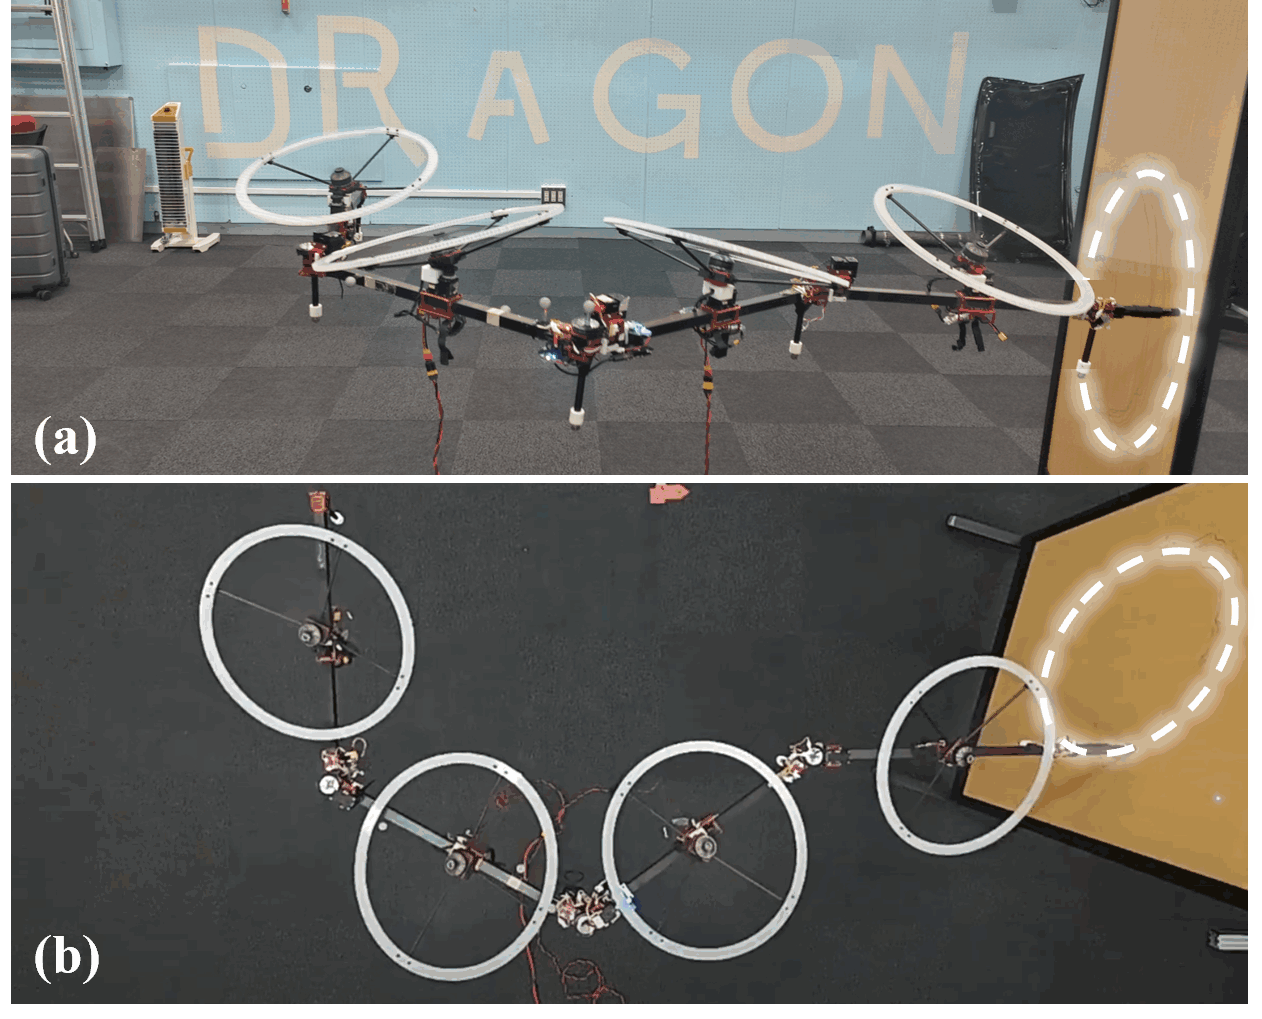
\includegraphics[width=\linewidth]{figures/chapter1/main_figure.png}
  \caption{A multi-link aerial robot is tracking a circular trajectory on a sloped board while maintaining contact. The desired trajectory is marked by a white dashed line. (a) Side view. (b) Top view.}
  \label{fig:main_figure}
  \vspace{-7mm}
\end{figure}

To execute tasks in such kind of interaction scenarios, previous work has commonly adopted force-control strategies such as impedance control and admittance control \cite{ollero_2021_past}. However, they each have their own advantages and disadvantages. Impedance control performs well in regulating interaction forces and resisting external force disturbances, but typically exhibits limited adaptability to changing contact geometry. In contrast, admittance control is effective in adapting to geometric variations, but is generally less robust against large interaction force disturbances. These differences originate from the complementary yet opposite causal relationships of impedance and admittance control paradigms \cite{ott_2010_unified}. Consequently, contact-rich tasks that simultaneously require disturbance rejection and adaptation to uncertain surface geometry cannot be reliably addressed by either approach alone, naturally motivating a combination of both control principles to achieve resilient and adaptive interaction capabilities.

Previous researches have pay a lot of attentions on impedance control or admittance control on aerial robot. However, currently, there is not a control method combined them together, while obviously we need both of their abilities. This is because achieving such a combination is not trivial. Due to the opposite causality of impedance and admittance control, a single actuation source cannot independently realize both interaction objectives and generally requires additional coordination mechanisms \cite{ott_2010_unified}. Conventional aerial robot platforms, which rely exclusively on rotor thrusts, inherently possess only a single actuation source and are therefore limited in their ability to simultaneously exploit the complementary properties of the two paradigms.


Luckily, if the aerial robot is mounting a robotic arm or is a multi-link aerial robot, this problem can be solved. The current situation is, although some aerial manipulation platforms (e.g., \cite{lippiello_2012_cartesian, cataldi_2016_impedance}) introduce joint actuation and therefore provide additional actuation source, existing studies have not leveraged this structural characteristic to simultaneously employ both impedance and admittance control. This limitation further motivates the design of our control strategy. Considering the future scalability of this control framework, we chose to use the multi-link aerial robots as the development platform, and combine impedance and admittance control simultaneously.

In this work, we propose a novel hybrid impedance--admittance control enabled by multi-link aerial robots, which exploits the two independent actuation sources of the robot by assigning them distinct control roles. In particular, rotor thrusts govern the global motion of the platform, whereas the joint actuators regulate the end-effector pose relative to the platform's body. This structure enables impedance control to be implemented through rotor thrusts and admittance control through joint actuation, allowing both paradigms to be realized simultaneously on a single aerial platform. Within the proposed framework, impedance control regulates the aerial robot's center-of-gravity (CoG) motion to achieve disturbance-resilient interaction, while admittance control adjusts joint angles to accommodate unmodeled surface geometric and contact-induced variations. Through this division of roles, the proposed strategy enables resilient and adaptive sliding along unknown surfaces. The task execution process is illustrated in Fig.~\ref{fig:main_figure}.


%%%%%%%%%%%%%%%%%%%%%%%%%%%%%%%%%%%%%%%%%%%%%%%%%%%%%%%%%%%%%%%%%%%%%%%%%%%%%%%%
\section{Previous Research}

\subsection{Morphologies of aerial robot for aerial manipulation}
% Considering that the aeria manipulation is directly derived from the ground manipulation field, the morphology of the manipulatiors attached in the aerial robot is usually very similar with those in the ground robot. Obviously, we can used the mechanical design and control method that have been demonstrated in the ground robot field.
%The morphology is very important for the aerial manipulation\cite{ollero_2021_past}. 
We can briefly divide the morphologies of aerial manipulation into four types: single rigid body morphology, parallel morphology, series morphology and other specific morphology like multi-link aerial robot as illustrated in Fig.~\ref{fig:morphologies}. These morphologies have their own features for different type of tasks.

The single rigid body morphology is just install a rod or a stick on the aerial robot, and the manipulator usually keeps static to the aerial robot. This kind of morphology is very simple, we don't need to think about how to control the end effector itself. 
By mainly controling the aerial robot itself to provide degree of freedom for the end effector, the rigid manipulator is used for task like push-and-slide and peg-in-hole. 
%The end effector is usually a pad that installed with sensors, or a roller to move in the surface %smoothly. 
The main requirement is the pose of manipulator, and it is ragulate by aerial robot's pose.
In the recent research. For example Bodie et al. \cite{bodie_2020_active} uses a static end effector to inspect bridge. Brunner et al. \cite{brunner_2022_planning} realized to operate an articulated door. 
%Actually, they did not use the manipulator it self to do the tasks.
However, for more complicated tasks, the rigid manipulator may be not enough. Meanwhile, the rigid manipulator do not have extra d.o.f, so if the requirements need more, this type is not good. 


The parallel morphology is defined as an aerial robot mounted with a delta manipulator. Since the delta manipulator has the adventages of low inertia, high stiffness and fast response due to its mechnical structure, the paraller morphology can realize high-speed motion and accurate position control. 
Due to these adventages, a few researchers have used such kind of morphology. Guo et al. \cite{guo_2024_flying} performed calligraph on a board with the parallel morphology,showing the potential of this morphology for precise manipulation tasks.Deng et al. \cite{deng_2025_whole} realized high speed manipulation like push objects and grasping object, indicating the ability of achieve fast motion requirements.
The above application demonstrate that the parallel morphology can perform well in high precision and high speed requirements. However, since the surface sliding tasks usually requires large work space that the delta manipulator do not have, this morphology will struggle when faced with a wider range of surface geometry variations.

\begin{figure}[t]
  \centering
  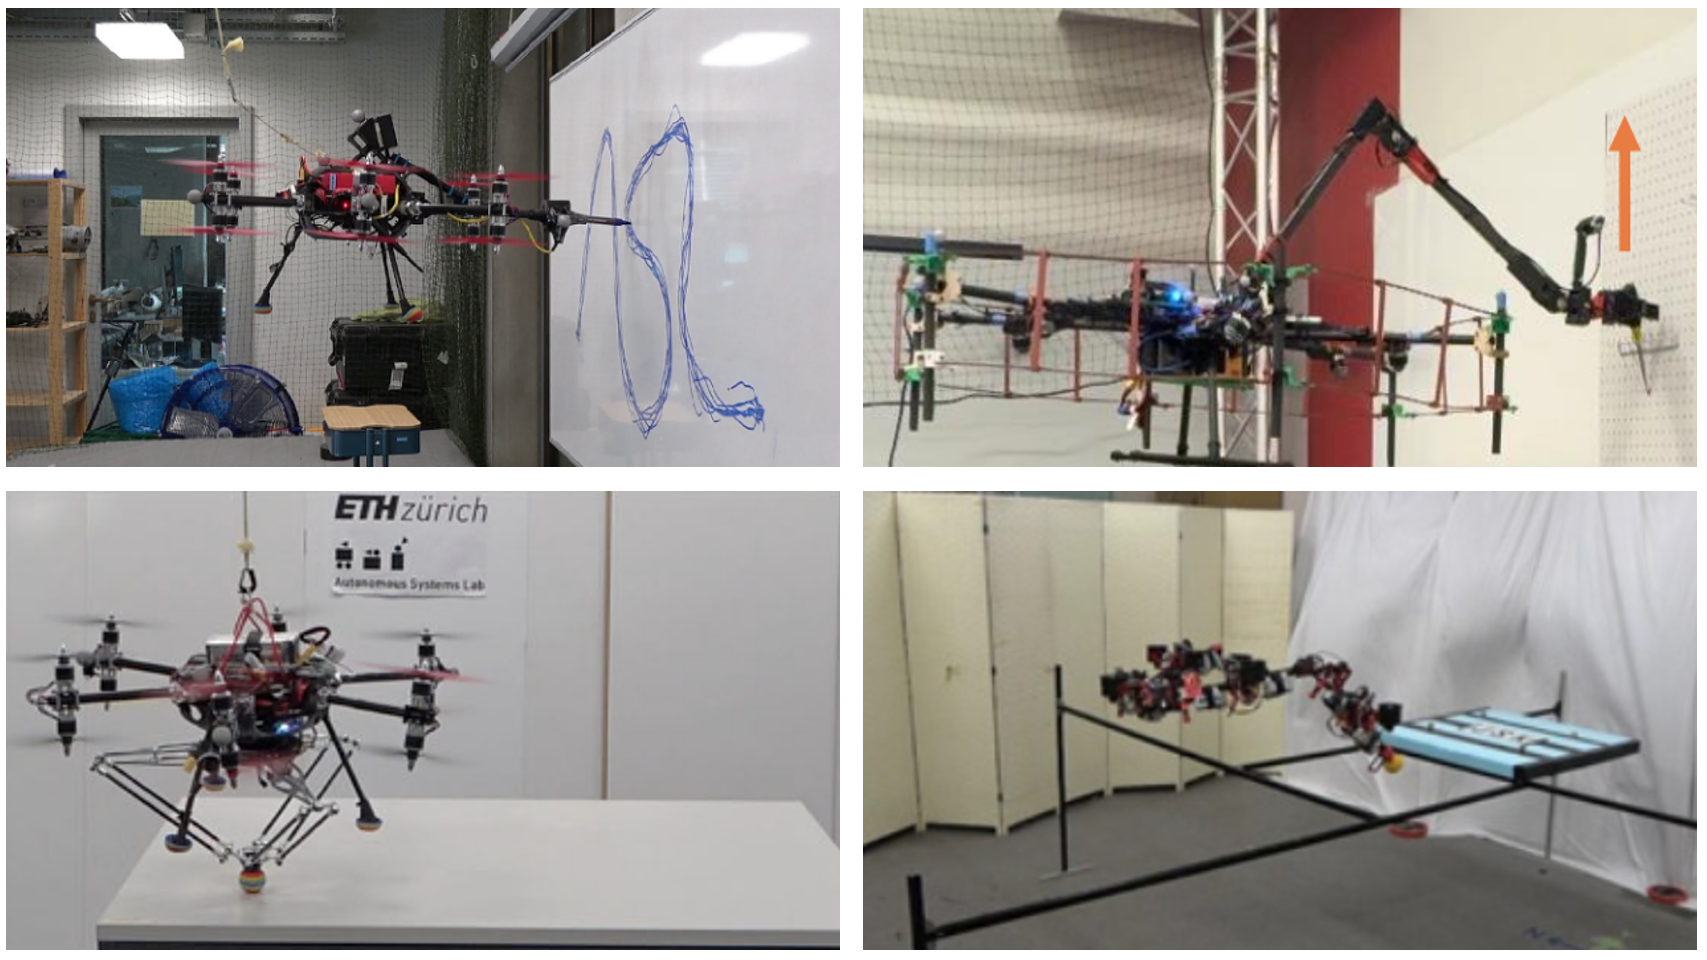
\includegraphics[width=\linewidth]{figures/chapter1/morphologies.png}
  \caption{Four morphologies of aerial robots. (a) Static end effector. (b) serial manipulator. (c) delta manipulator. (d) multi-link aerial robot}
  \label{fig:morphologies}
  \vspace{-7mm}
\end{figure}

The serial morphology is defined as an robotic arm manipulator mounted on an aerial robot. The serial structures of robotic arm provides large work space. In contrast to the parallel morphology, the serial morphology is usually used in tasks requiring large working space and obstacle avoidance ability. 
Move a robotic arm to an aerial robot is an intuitive idea, therefore a lot of researches realize it. He et al. \cite{he_2025_flying} used serial arm to draw a relative large figure on a board. 
Lee et al. \cite{lee_2025_autonomous} realized SE(3) operation like peg-in-hole in a large scenario. 
Both demonstrated that the serial morphology possesses strong operational capabilities and potential.
Due to the multi-DOF structure, both serial morphology and multi-link morphology provide flexible manipulation capabilities for aerial robots.


%Too support the hole arm, it needs high quality rotor, which will also bring high weight.

The mutli-link aerial robot itself can be called multi-link morphology. This type of morphology can be regarded as a flying robotic arm, so it has all the strengths of serial morphology. Meanwhile, the multi-link aerial robot can trans trought narrow gap that the normal aerial robot can not achieve.
The extra d.o.f of multi-link aerial robot can also help it do more things. Sugito et al. \cite{sugito_2022_aerial} used multi-link aerial robot to push a door. Shi et al. \cite{shi_2020_aerial} used multi-link aerial robot to grasp a box. We already know the morphology with serial structures has the ability in surface sliding tasks. However until now, the multi-link aerial robot has not been used in the surface sliding tasks. THerefore in this work, considering the morphology features, we develop the control framework for the multi-link aerial robot.


In conclusion, the morphologies of aerial robots would influence the abilities: parallel robotic arms usually used for agile manipulation tasks, while the series arms are used for large working space tasks. When it comes to complicated aerial manipulation tasks like surface sliding tasks, multi-link aerial robot is a good choice.




\subsection{control method used in aerial manipulation}
For more and more interaction aerial manipulation tasks, it is important to introduce force-control methods. Previous work has commonly adopted force-control strategies such as impedance control and admittance control \cite{ollero_2021_past}. 

Both impedance and admittance control can be considered as can be considered as general impedance control \cite{valency_2003_accuracy}. The concept of impedance control is put forward by Hogan \cite{hogan_1984_impedance}. In his paper, the environment should be considered as an admittance, therefore if the robot performs like an impedance, the power flow will be reasonable. Currently, the conception of impedance and admittance controller becomes a little different. If the system perform like a compliant second order system, it can be called as impedance control. In detail, the impedance control wishes the system performs like a real second order system, the main idea of it is to design a second order system. On the other hand, the admittance control tries to imitate a second order system, whose position almost follow the design system. Transparently, both impedance and admittance control performs similarly, but their causalities are completely opposite. Due to their concern object, The impedance control is better used in the force control actuator, and the admittance control has better used in position control actuator, or perform as a filter to provide reference position command for lower layer controllers.

Among these strategies, impedance control has been extensively explored for aerial robots. 
For the beginning of aerial manipulation research, the impedance control method was used \cite{ollero_2021_past}.
Forte et al. \cite{forte_2012_impedance} calculated the 3D impedance control for a single rigid body aerial robot, and Lippiello et al. \cite{lippiello_2012_cartesian} put forward the impedance equation of an aerial robot with a serial arm. In his paper, the aerial robot itself and the 3-dof robotic arm is set different dynamic parameters, which also gives this thesis inspiration. After those work introduce impedance control into aerial manipulation tasks, the community more focused on the effect impedance control can realize.
In recent years, the impedance control has been used in more complicated tasks.
Bodie et al. \cite{bodie_2020_active} introduced a six-DOF axis-selective impedance controller capable of adjusting impedance gains based on surface proximity. In this work, the impedance control is considered as the adjusting part. This work realized sliding on the surface, following a specific trajectory, which can be used for bridge inspection task.
Zhang et al. \cite{zhang_2022_learning} employed learning-based techniques to adapt the impedance parameters, which helps the aerial robot sliding on an uneven plane. Both work pay attention to use impedance control as a adjusting part to adapt to the unknown external environment that has different force requirements. 
We can see that using impedance control in aerial robot is relatively mature. However, current literatures are mainly focusing on designing a useful control framework instead analyzing how the impedance controller perform in different tasks, or analyzing how the parameters effect the performance of aerial manipulation.
These methods can effectively respond to external force disturbances through gain modulation. However, there is limited evidence that they remain effective in environments with uneven or irregular surfaces by adapt to the geometric variations. 

In addition to impedance approaches, admittance control has also been applied in aerial manipulation tasks. 
Someone uses admittance control as a filter, and the framework use PID control as the inner controller.
Ryll et al. \cite{ryll_2019_6d} enabled an aerial robot to follow variations in the contact-plane geometry, yet the induced lateral force disturbances caused noticeable rotational deviations.
Cataldi et al. \cite{cataldi_2016_impedance} used an admittance filter to calculate the reference values.

The admittance control is less than impedance control.

In our framework ,admittance control is more like controlling a robotic arm instead of an aerial robot. Therefore, we will introduce admittance control used in controlling robotic arms. 
Admittance control has been used in robotics arm like




In conclusion, while these studies demonstrate the potential of impedance- or admittance-based approaches for aerial manipulation tasks in interaction scenarios, each method inevitably inherits the limitations of its underlying control principle.
This thesis tries to combine these two controllers together on the same platform in order to gain both of their strengths.
\subsection{cooperative aerial manipulation}
In the surface sliding task, besides the contact requirements, there must be some secondary task, such as taking photos or keep the cable stable. This kind of requirements are not the essential problem in surface sliding, but it will effect whether we can use the whole system into the real application. In this thesis, we can also answer how to use the multi-link structure to achieve the secondary requirements.

A similar solution for the secondary requirements is the cooperative aerial manipulation. In this kind of aerial manipulation, multi aerial robots can take part in the task and be respond to some requirements. The cooperative aerial manipulation can be divided into two types. First is all of the aerial robots share the some ability, like two aerial robot work together to grasp a long stick. Second is the aerial robots have different requirements. We can image a dual aerial robots system with a prior robot and a secondary robot, the prior robot need to completed the contact tasks, and the secondary robot help it in photography. Transparently, the secondary aerial robot also has special control requirements, so we can use the method in the first type, for example to image a virtual stick between the contact point and the photography point, and these two aerial robots need to grasp the virtual stick. By using the same control method, these type of cooperative aerial manipulation tasks can also be solved. So in our view, to solve the secondary requirements, we must research for the cooperative aerial manipulation.

Most of the cooperative aerial manipulation pay attention to two aerial robots. The fundamental of the cooperative aerial manipulation is to control two frames trajectories simultaneously. Our multi-link aerial robot can also do that by using its two ends. Additionally, the double aerial robots manipulation must has problems like: the two robots need to wireless connect to transport the information. Meanwhile, the two ends of multi-link aerial robot is connected by physical structures, which must be more reliable compared to the double aerial robot system.

Caccavale et al. \cite{caccavale_2015_cooperative} tried to used impedance control to adjust two aerial robots in order to grasp a stick. We can imitate it.

%%%%%%%%%%%%%%%%%%%%%%%%%%%%%%%%%%%%%%%%%%%%%%%%%%%%%%%%%%%%%%%%%%%%%%%%%%%%%%%%
\section{The construction of the thesis}

This thesis investigates the force control method of multi-link aerial robot. The overall structure of the thesis is organized as follows.


\begin{itemize}
	\item Chapter 1 introduces the research background and motivation of this study, reviews related work about morphologies of aerial robots, force control methods used in aerial manipulation, and the current situation of cooperative aerial manipulation. Based on above discussion, the motivation, objectives and contributions of this thesis are introduced.
	\item Chapter 2 presents the mechanical design of two different types of multi-link aerial robots. The modeling process is introduced.
	\item Chapter 3 introduces the basic concepts of impedance control and admittance control, analyzes how the impedance control can redesign the dynamic parameters of a system, and how the admittance influence the distance between the CoG and the end effector. The effects of the hybrid controller is proved on the 2D multi-link aerial robot platform Hydrus Xi.
	\item Chapter 4 introduces how to combined impedance control and admittance control together on the same system. The admittance control is used for adjust the internal configuration of the aerial robot, while perform adaptation to the external geometric variations. The effects of the intergrated hybrid controller is proved on the 3D multi-link aerial robot platform DRAGON.
	\item Chapter 5 presents experimental results.
	\item Finally, Chapter 6 concludes the thesis by summarizing the main findings and contributions of this work and outlining directions for future research
\end{itemize}



\chapter{Preliminary}
%%%%%%%%%%%%%%%%%%%%%%%%%%%%%%%%%%%%%%%%%%%%%%%%%%%%%%%%%%%%%%%%%%%%%%%%%%%%%%%%

In this chapter, The notation used throughout this thesis, the modeling of multi-link aerial robots, and the external wrench estimation method will be introduced. In the modeling part, two types of multi-link aerial robots will be presented. One is the underactuated multi-link aerial robot Hydrus Xi, which can achieve 2D deformation while retaining the overall actuation of a conventional quadrotor. The other is the overactuated multi-link aerial robot DRAGON, which can deform in a 3D workspace. The basic constructions, dynamics and allocation modeling processes will be introduced.


\section{Notation}
In this thesis, we denote scalars by regular font $x \in \mathbb{R}$, vectors by bold lowercase $\boldsymbol{x} \in \mathbb{R}^n$, and matrices by bold uppercase $\boldsymbol{X} \in \mathbb{R}^{m \times n}$. A vector expressed in frame $\{A\}$ is written as $^A\boldsymbol{p}$, and the rotation matrix from frame $\{A\}$ to frame $\{B\}$ is denoted as $^A\boldsymbol{R}_B$.
Also, $\{W\}$ represents the world frame, and $\{C\}$ represents the CoG frame. For each link $i\in\{1,2,3,4\}$, $\{F_i\}$ and $\{G_i\}$ denote the thrust frame and gimbal roll frame of the corresponding gimbal module, while $\{L_i\}$ denotes the corresponding link frame.

%%%%%%%%%%%%%%%%%%%%%%%%%%%%%%%%%%%%%%%%%%%%%%%%%%%%%%%%%%%%%%%%%%%%%%%%%%%%%%%%

\section{Modeling of Multi-Link Aerial Robots}

\subsection{General Description of Multi-Link Aerial Robots}
The multi-link aerial robots consist of multiple serially connected links for deformation. Two typical multi-link aerial robots are shown in Fig.~\ref{fig:multi-link}. The relative angles between the adjacent links can be changed through joint actuation, enabling robotic arm-like movements in the air. To realize the dexterous aerial motion, rotors are arranged on the gimbal modules, which can change the thrust direction of the rotors depending on the gimbal types, thereby achieving vectoring thrust. Each link is equipped with one gimbal module. The thrust direction of each rotor can be adjusted by the gimbal module to maintain stable flight and generate the required wrench for aerial manipulation. In particular, the required thrust direction varies with the joint configuration, even when the desired flight condition remains unchanged.


\subsection{Dynamic Model}

Using the notation defined above, the dynamics of the multi-link aerial robots at their CoG, derived from the Newton--Euler equations, are given by:
\begin{subequations}
\label{eq:dynamics}
\begin{align}
    m(^W\!\ddot{\boldsymbol{p}}+\boldsymbol{g})&= {^W\!\boldsymbol{f}_{cmd}} + {^W\!\boldsymbol{f}_{ext}}, \\[2pt]
    \boldsymbol{I}{^C\!\dot{\boldsymbol{\omega}}}+{^C\!\boldsymbol{\omega}} \times \boldsymbol{I}{^C\!\boldsymbol{\omega}}&={^C\!\boldsymbol{\tau}_{cmd}} + {^C\!\boldsymbol{\tau}_{ext}},
\end{align}
\end{subequations}
where $m$ is the total mass, $\boldsymbol{I}$ is the total inertia matrix expressed in frame $\{C\}$, $^W\boldsymbol{p}$ is the position of the oringinal point of  the CoG frame $\{C\}$ in the world frame $\{W\}$, $^{C}\boldsymbol{\omega}$ is the angular velocity of the CoG frame $\{C\}$ expressed in frame $\{C\}$, $\boldsymbol{g}$ is the gravitational acceleration, ${^W\!\boldsymbol{f}_{cmd}}$, ${^C\!\boldsymbol{\tau}_{cmd}}$ and ${^W\!\boldsymbol{f}_{ext}}$, ${^C\!\boldsymbol{\tau}_{ext}}$ denote the command force and torque, and the external force and torque, respectively. Since the joint angles and thrust directions vary during motion, the inertia matrix is configuration dependent and may vary accordingly. Here, we consider the multi-link aerial robot as a quasi-static system, meaning that the variations in the inertia matrix caused by joint and thrust-vectoring motions are negligible within a single control period \cite{zhao_2021_singularity, zhao_2023_versatile}.


\begin{figure}[t]
    \centering
    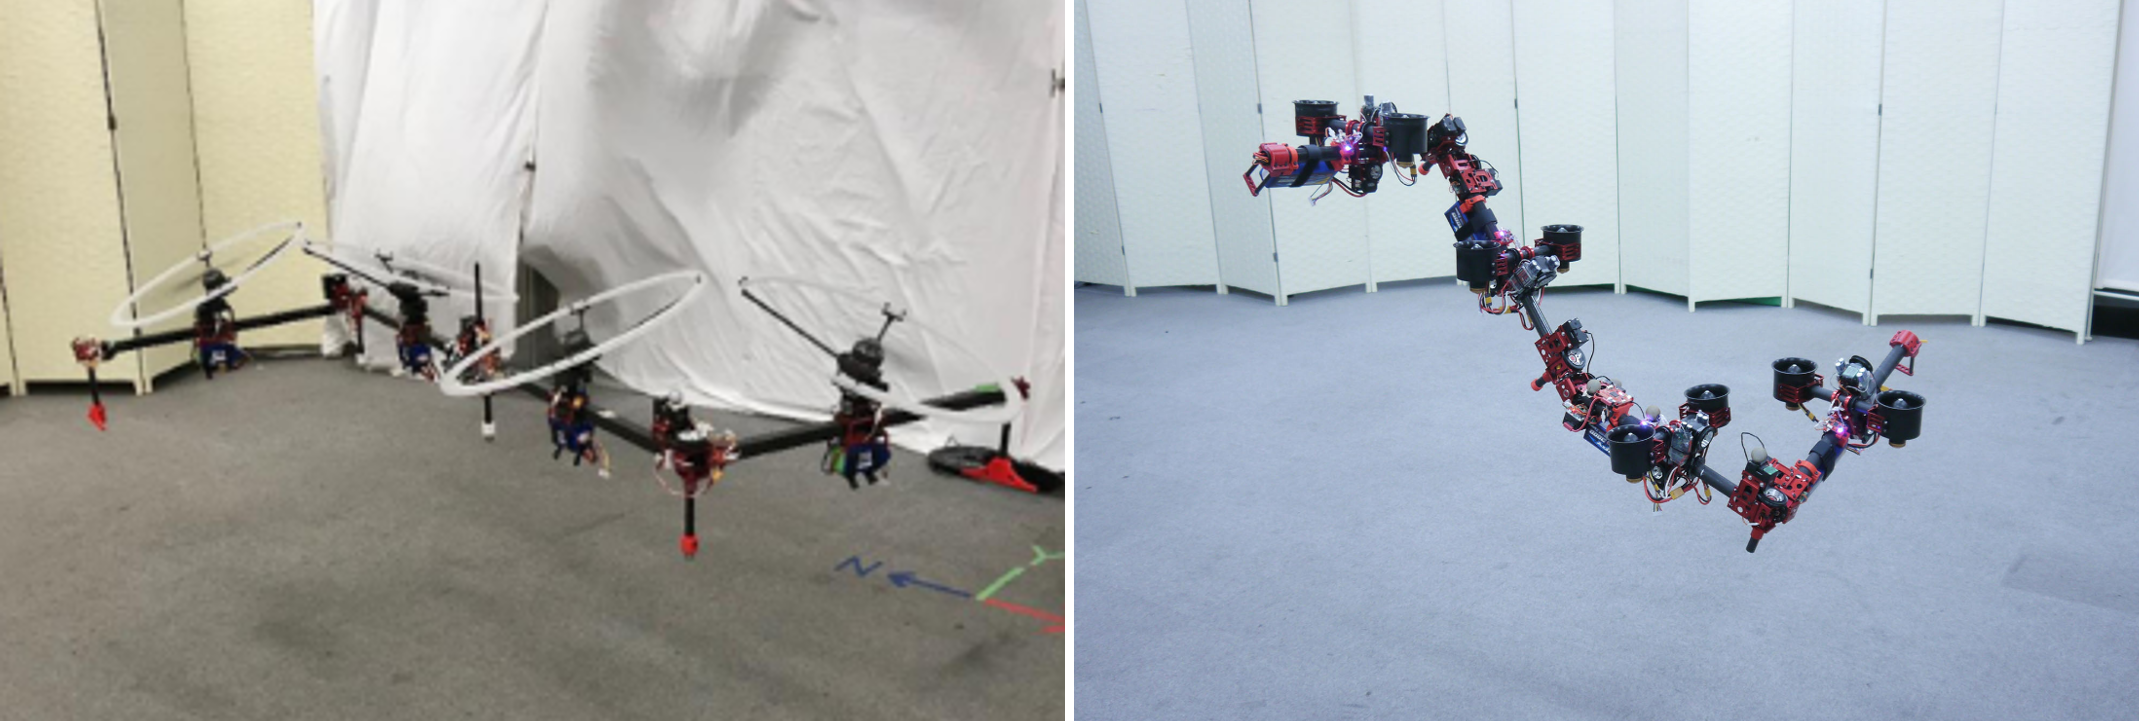
\includegraphics[trim={0cm 0cm 0cm 0cm}, clip, width=\linewidth]{figures/chapter2/multi-link.png}
    \caption{Photographs of the multi-link aerial robots. (a): underactuated multi-link aerial robot Hydrus Xi \cite{zhao_2021_singularity}. (b): overactuated mutli-link aerial robot DRAGON \cite{zhao_2018_design}.}
    \label{fig:multi-link}
\end{figure}

\subsection{Allocation}
The command force ${^W\boldsymbol{f}_{cmd}}$ and the command torque ${^{C}\boldsymbol{\tau}_{cmd}}$ are obtained by aggregating the contributions of the rotors mounted on the gimbal modules, whose individual forces and torques are expressed in frame $\{C\}$. We compute each module's contribution as follows:
\begin{equation}
\label{eq:allocation for force}
    {^C\!\boldsymbol{f}_i}=\lambda_i^C\!\boldsymbol{R}_{F_i}\boldsymbol{b}_3,
\end{equation}

\begin{equation}
\begin{aligned}
\label{eq:allocation for torque}
    {^C\!\boldsymbol{\tau}_i}&=^C\!\!\boldsymbol{p}_{F_i}\times^C\!\!\boldsymbol{f}_i+\kappa_i ^C\!\boldsymbol{f}_i\\
    &=\lambda_i(^{C}\boldsymbol{\hat{p}}_{F_i}+\kappa_i\boldsymbol{E}_3)^C\boldsymbol{R}_{F_i}\boldsymbol{b}_3.
\end{aligned}
\end{equation}
Here, $i\in\{1,2,3,4\}$ since the multi-link aerial robots considered in this thesis consist of four links. The joint angles and thrust directions determine $^{C}\boldsymbol{R}_{F_i}\in \mathbb{R}^{3\times3}$ and $^{C}\boldsymbol{p}_{F_i}\in \mathbb{R}^3$, which denote the rotation matrix and the position vector of the rotor frame $\{F_i\}$ with respect to the CoG frame $\{C\}$. The rotor frame $\{F_i\}$ is attached to the rotor mount, and the thrust force $\lambda_i$ is along the $z$ axis of $\{F_i\}$. The vector $\boldsymbol{b}_3 = \begin{bmatrix}0 & 0 & 1\end{bmatrix}^{\mathrm{T}}$ is a unit vector and $\kappa_i$ is the coefficient associated with the rotor drag moment. The operator $\hat{\cdot}$ converts a vector into a skew-symmetric matrix, and $\boldsymbol{E}_3$ denotes the $3 \times 3$ identity matrix. 

Using \eqref{eq:allocation for force} and \eqref{eq:allocation for torque}, the mapping from the thrust vector $\boldsymbol{\lambda} = \begin{bmatrix}\lambda_1 & \lambda_2 & \lambda_3&\lambda_4\end{bmatrix}^{\mathrm{T}}$ to the command wrench is given by:
\begin{equation}
\label{eq:allocation for wrench}
^C\!\boldsymbol{w}_{cmd}
=
\begin{pmatrix}
^C\!\boldsymbol{f}_{cmd} \\
^C\!\boldsymbol{\tau}_{cmd}
\end{pmatrix}
=
\sum_{i=1}^{4}
\begin{pmatrix}
^C\!\boldsymbol{f}_i \\
^C\!\boldsymbol{\tau}_i
\end{pmatrix} 
=\begin{pmatrix}
\boldsymbol{Q}_t \\
\boldsymbol{Q}_r
\end{pmatrix}\boldsymbol{\lambda},
\end{equation}
where $\boldsymbol{Q}_t \in \mathbb{R}^{3\times4}$ and $\boldsymbol{Q}_r\in \mathbb{R}^{3\times4}$ denote the translational and rotational components of the allocation matrix, respectively. The command force in the world frame can be obtained by $^W\!\boldsymbol{f}_{cmd} = ^W\!\!\!\boldsymbol{R}_C{}^C\!\boldsymbol{f}_{cmd}$.

In this thesis, the allocation matrices $\boldsymbol{Q}_t$ and $\boldsymbol{Q}_r$ depend on the joint angles and thrust directions. We use the optimization method introduced in \cite{zhao_2021_singularity} or an iterative solution using gradients based on an optimization method introduced in \cite{zhao_2023_versatile} to calculate the thrust directions and the gimbal angles automatically. 


\subsection{Underactuated Configuration: Hydrus Xi}
The underactuated multi-link aerial robot Hydrus Xi \cite{zhao_2021_singularity} is shown in Fig.~\ref{fig:hydrus_model}. The platform consists of four links, each of which carries an independent gimbal module. The robot employs a serial-link structure with one rotational degree of freedom per joint, whose joint axes are aligned in parallel. Here, $q_i$ is used to represent the $i$th joint angle. Each gimbal module features a fixed tilt angle $\beta$ and a 1-DoF yaw rotation mechanism to vector the thrust direction. The corresponding rotation angle, referred to as the vectoring angle, is denoted by $\psi_i$. The design of the gimbal module was originally developed in \cite{anzai_2019_design}. Besides the joint angles, Hydrus Xi has eight actuation inputs: four rotor thrusts $\boldsymbol\lambda$ and four vectoring angles $\boldsymbol\psi$. However, to maximize the possible torque generated under the current configuration, the vectoring angles $\boldsymbol\psi$ are automatically adjusted through an optimization method \cite{zhao_2021_singularity}. Therefore, only the four rotor thrusts remain as direct control inputs, making Hydrus Xi an underactuated system.


\begin{figure}[t]
    \centering
    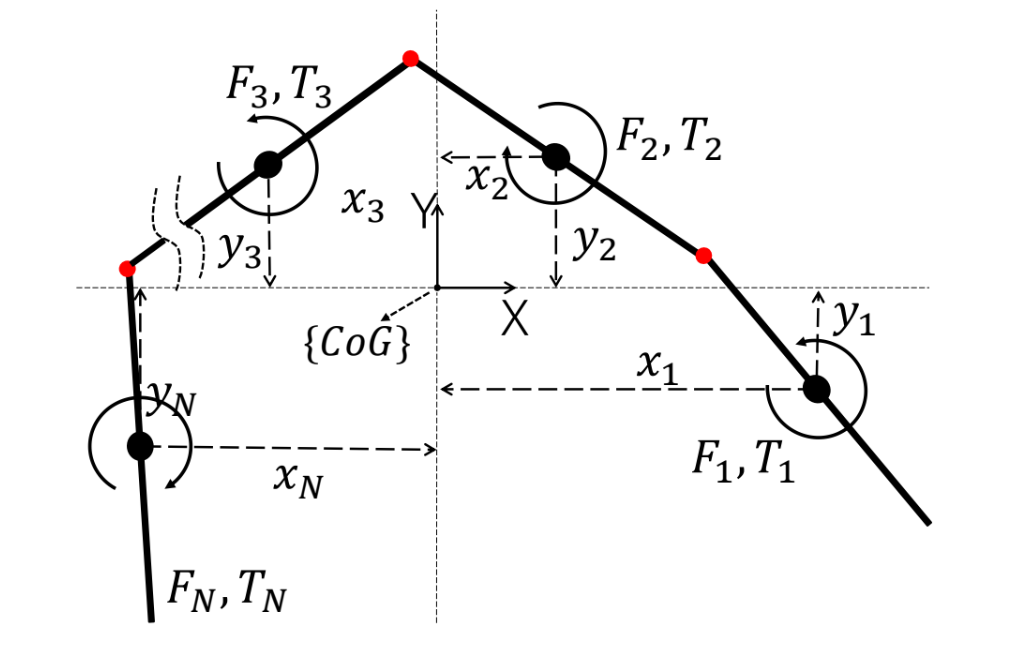
\includegraphics[trim={0cm 0cm 0cm 0cm}, clip, width=\linewidth]{figures/chapter2/hydrus_model.png}
      \caption{Model of the underactuated multi-link aerial robot Hydrus Xi. $\{L_i\}$ denotes the link frame, while $\{F_i\}$ denotes the thrust frame whose $z$ axis is aligned with the thrust direction. The tilt angle between $z$ axes of $\{L_i\}$ and $\{F_i\}$ is $\beta$, and the vectoring angle is $\psi_i$. }
    \label{fig:hydrus_model}
\end{figure}


Note that the transform from $\{C\}$ to $\{F_i\}$ changes due to the joint angles $q_i$ and the vectoring angles $\psi_i$. Therefore, the command equations (\ref{eq:allocation for force}), (\ref{eq:allocation for torque}) and (\ref{eq:allocation for wrench}) can be rewritten as

\begin{equation}
\label{eq:allocation for force hydrus}
    {^C\!\boldsymbol{f}_i}=\lambda_i^C\!\boldsymbol{R}_{F_i}(\boldsymbol{q},\boldsymbol{\psi})\boldsymbol{b}_3,
\end{equation}

\begin{equation}
\begin{aligned}
\label{eq:allocation for torque hydrus}
    {^C\!\boldsymbol{\tau}_i}&=^C\!\!\boldsymbol{p}_{F_i}(\boldsymbol{q},\boldsymbol{\psi})\times^C\!\!\boldsymbol{f}_i+\kappa_i ^C\!\boldsymbol{f}_i\\
    &=\lambda_i(^{C}\boldsymbol{\hat{p}}_{F_i}(\boldsymbol{q},\boldsymbol{\psi})+\kappa_i\boldsymbol{E}_3)^C\!\boldsymbol{R}_{F_i}(\boldsymbol{q},\boldsymbol{\psi})\boldsymbol{b}_3,
\end{aligned}
\end{equation}

\begin{equation}
\label{eq:allocation for wrench hydrus}
^C\!\boldsymbol{w}_{cmd}
=
\begin{pmatrix}
^C\!\boldsymbol{f}_{cmd} \\
^C\!\boldsymbol{\tau}_{cmd}
\end{pmatrix}
=
\sum_{i=1}^{4}
\begin{pmatrix}
^C\!\boldsymbol{f}_i \\
^C\!\boldsymbol{\tau}_i
\end{pmatrix} 
=\begin{pmatrix}
\boldsymbol{Q}_t(\boldsymbol{q},\boldsymbol{\psi}) \\
\boldsymbol{Q}_r(\boldsymbol{q},\boldsymbol{\psi})
\end{pmatrix}\boldsymbol{\lambda},
\end{equation}
where $\boldsymbol{Q}_t(\boldsymbol{q},\boldsymbol{\psi}) $ and $\boldsymbol{Q}_r(\boldsymbol{q},\boldsymbol{\psi})$ are functions of the joint angles $\boldsymbol q$ and vectoring angles $\boldsymbol\psi$.



\subsection{Overactuated Configuration: DRAGON}
The overactuated multi-link aerial robot DRAGON \cite{zhao_2018_design, zhao_2023_versatile} is shown in Fig.~\ref{fig:dragon_model}. The platform also consists of four links, each of which is equipped with an independent gimbal module. The robot employs a serial-link structure with two rotational degrees of freedom between adjacent links, realized by two orthogonal rotational joints. Here, $q_i$ is used to represent the $i$th joint angle. Each gimbal module has two gimbal angles, $\phi_i$ and $\theta_i$, which provide two degrees of freedom for changing the thrust direction relative to the corresponding link. More details of the robot structure can be found in \cite{zhao_2018_design}. In DRAGON's case, there are 12 actuation inputs excluding the joint angles, including four rotor thrusts $\boldsymbol{\lambda}$, four gimbal roll angles $\boldsymbol{\phi}$, and four gimbal pitch angles $\boldsymbol{\theta}$. All of them need to be determined as control inputs. With these redundant actuation inputs, DRAGON is an overactuated system.



\begin{figure}[t]
    \centering
    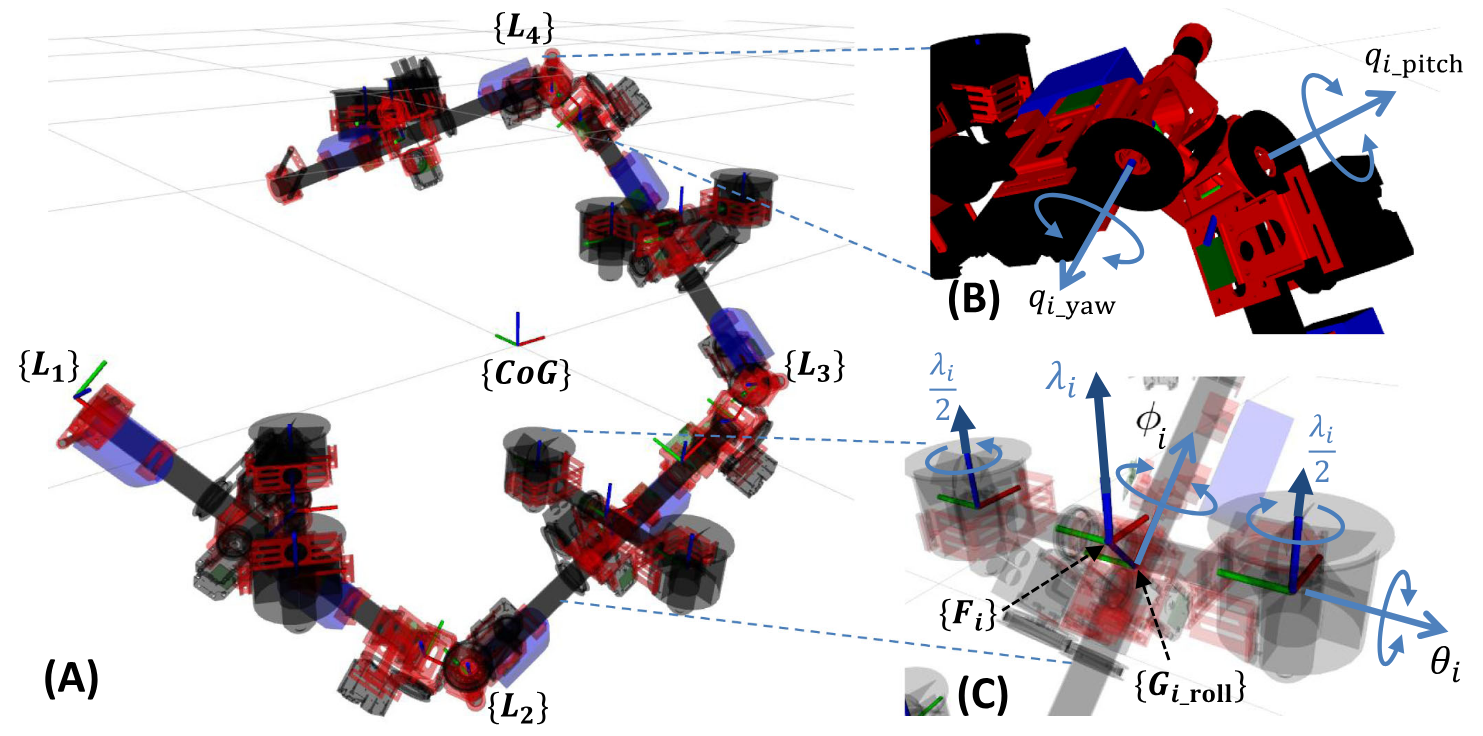
\includegraphics[trim={0cm 0cm 0cm 0cm}, clip, width=\linewidth]{figures/chapter2/dragon_model.png}
    \caption{Model of the overactuated multi-link aerial robot DRAGON. (a) Kinematic model of DRAGON, with $\{L_i\}$ denoting the link frame. (b) Two-DoF joint module with orthogonal yaw and pitch axes ($q_{i\_yaw}$, $q_{i\_pitch}$). (c) Two-DoF thrust-vectoring apparatus with gimbal angles $\theta_i$ and $\phi_i$. $\{G_i\}$ denotes the intermediate frame (gimbal roll frame) after the $\phi_i$ rotation, while $\{F_i\}$ denotes the thrust frame whose $z$ axis is aligned with the thrust direction.}
    \label{fig:dragon_model}
\end{figure}




In DRAGON's case, the command equations (\ref{eq:allocation for force}), (\ref{eq:allocation for torque}) and (\ref{eq:allocation for wrench}) can be rewritten as 

\begin{equation}
\label{eq:allocation for force dragon}
    {^C\!\boldsymbol{f}_i}=\lambda_i^C\!\boldsymbol{R}_{L_i}(\boldsymbol{q})^{L_i}\boldsymbol{R}_{G_i}(\phi_i)^{G_i}\boldsymbol{R}_{F_i}(\theta_i)\boldsymbol{b}_3=\lambda_i^{C}\!\boldsymbol{u}_i.
\end{equation}

\begin{equation}
\label{eq:allocation for torque dragon}
    {^C\!\boldsymbol{\tau}_i}=\lambda_i^{C}\!\boldsymbol{p}_{F_i}(\boldsymbol{q}, \phi_i ) \times ^{C}\!\!\boldsymbol{u}_i=\lambda_i^{C}\!\boldsymbol{v}_i.
\end{equation}

\begin{equation}
\label{eq:allocation for wrench dragon}
^C\!\boldsymbol{w}_{cmd}=\begin{pmatrix}
^C\!\boldsymbol{f}_{cmd} \\
^C\!\boldsymbol{\tau}_{cmd}
\end{pmatrix}
=
\sum_{i=1}^{4}
\begin{pmatrix}
^C\!\boldsymbol{f}_i \\
^C\!\boldsymbol{\tau}_i
\end{pmatrix} 
=\boldsymbol{Q}(\boldsymbol{q}, \boldsymbol{\phi}, \boldsymbol{\theta})\boldsymbol{\lambda},
\end{equation}
where 
\begin{equation}
\label{eq:Q dragon}
\boldsymbol{Q} = 
\begin{pmatrix}
^C\!\boldsymbol{u}_1&^C\!\boldsymbol{u}_2&^C\!\boldsymbol{u}_3&^C\!\boldsymbol{u}_4\\
^C\!\boldsymbol{v}_1&^C\!\boldsymbol{v}_2&^C\!\boldsymbol{v}_3&^C\!\boldsymbol{v}_4
\end{pmatrix}.
\end{equation}
Here, $\boldsymbol{Q}(\boldsymbol{q}, \boldsymbol{\phi}, \boldsymbol{\theta}) \in \mathbb{R}^{6 \times 4}$ denotes the allocation matrix, which depends on the joint angles $\boldsymbol{q}$ and gimbal angles $\boldsymbol{\phi}$ and $\boldsymbol{\theta}$. For simplicity, its columns are denoted by $^C\boldsymbol{u}_i$ and $^C\boldsymbol{v}_i$.


%%%%%%%%%%%%%%%%%%%%%%%%%%%%%%%%%%%%%%%%%%%%%%%%%%%%%%%%%%%%%%%%%%%%%%%%%%%%%%%%
\section{External Wrench Estimation}

For both impedance control and admittance control, an external wrench is required in their respective formulations. An external wrench can be obtained either from a force sensor or through an estimation method. A force sensor generally measures the external wrench at its mounting location and introduces additional payload to the robot. To obtain the external wrench at the CoG without introducing additional payload from a force sensor, a momentum-based external wrench estimation method introduced in \cite{ruggiero_2014_impedance} is adopted in this framework. The wrench applied at the CoG is obtained as follows:

\begin{subequations}
\label{eq:external wrench estimation}
\begin{align}
 {^W\!\boldsymbol{\tilde{f}}_{ext}}=\boldsymbol{K}_{ti}(m^W\!\dot{\boldsymbol{p}}-\int({^W\!\boldsymbol{f}_{cmd}}-m\boldsymbol{g}+ {^W\!\boldsymbol{\tilde{f}}_{ext}})\mathrm{d}t),\\
 {^C\!\boldsymbol{\tilde{\tau}}_{ext}}=\boldsymbol{K}_{ri}(\boldsymbol{I}^C\!\boldsymbol{\omega}-\int({^C\!\boldsymbol{\tau}_{cmd}}-{^C\!\boldsymbol{\omega}} \times \boldsymbol{I}{^C\!\boldsymbol{\omega}} + {^C\!\boldsymbol{\tilde{\tau}}_{ext}})\mathrm{d}t),
\end{align}
\end{subequations}
where ${^W\!\boldsymbol{\tilde{f}}_{ext}}$ is the estimated external force, ${^C\!\boldsymbol{\tilde{\tau}}_{ext}}$ is the estimated external torque, and they can be assumed to be equal to the real external force ${^W\!\boldsymbol{f}_{ext}}$ and the real external torque  ${^C\!\boldsymbol{\tau}_{ext}}$, respectively. $\boldsymbol{K}_{ti} \in \mathbb{R}^{3\times3} $ and $\boldsymbol{K}_{ri} \in \mathbb{R}^{3\times3}$ are the estimator translational gain matrix and estimator rotational gain matrix, respectively.

Differentiating (\ref{eq:external wrench estimation}) and substituting (\ref{eq:dynamics}) into it yields a first-order low-pass filtered form: 
\begin{subequations}
\label{eq:external wrench estimation low-pass}
\begin{align}
 {^W\!\boldsymbol{\dot{\tilde{f}}}_{ext}}&=\boldsymbol{K}_{ti}({^W\!\boldsymbol{f}}_{ext}-{^W\!\boldsymbol{\tilde{f}}_{ext}}),\\
 {^C\!\boldsymbol{\dot{\tilde{\tau}}}_{ext}}&=\boldsymbol{K}_{ri}({^C\!\boldsymbol{\tau}_{ext}}-{^C\!\boldsymbol{\tilde{\tau}}_{ext}}).
\end{align}
\end{subequations}
This means that by increasing the parameters, the estimated data will follow the real data faster, but will also be more likely to introduce noise and lead to instability.

Note that \eqref{eq:external wrench estimation} estimates external forces and torques without using acceleration measurements, relying solely on the estimated linear and angular velocities. This means that the external wrench can be obtained using only the built-in IMU data.

%%%%%%%%%%%%%%%%%%%%%%%%%%%%%%%%%%%%%%%%%%%%%%%%%%%%%%%%%%%%%%%%%%%%%%%%%%%%%%%%
\section{Summary}
In this chapter, the notation used in this thesis is introduced first. The dynamics of the multi-link aerial robots are formulated based on the quasi-static assumption, from which the Newton--Euler equations are established. The difference between the underactuated and overactuated systems lies in the allocation process, which also affects the subsequent control design. A momentum-based external wrench estimation method is also introduced to estimate the external wrench acting on the robot. In the following chapters, we will introduce how the developed modeling equations and wrench estimation method are used to establish the control methods.


\chapter{Directional Hybrid Control}
%%%%%%%%%%%%%%%%%%%%%%%%%%%%%%%%%%%%%%%%%%%%%%%%%%%%%%%%%%%%%%%%%%%%%%%%%%%%%%%%
In this chapter, we will introduce the basis concept of impedance control and admittance control, as well as how can we realize it in the multi-link aerial robot. After that, the special setting on the 2D mutli-link aerial robot Hydrus Xi will be introduced. Finally, the hybrid impedance-admittance control will be introduced.
% We will discuss a new concept of impedance controller.
% also what should we consider when choosing the parameters in impedance and admittance controller
% \section{Motivation}

% The motivation for this hybrid impedance-admittance control framework is to provide both resilience and adaptivity when sliding on an unknown surface, where geometry and friction introduce significant uncertainties.
%%%%%%%%%%%%%%%%%%%%%%%%%%%%%%%%%%%%%%%%%%%%%%%%%%%%%%%%%%%%%%%%%%%%%%%%%%%%%%%%
\section{Framework Overview}

% \begin{figure}[h]
%     \centering
%     % \parbox{3in}
%     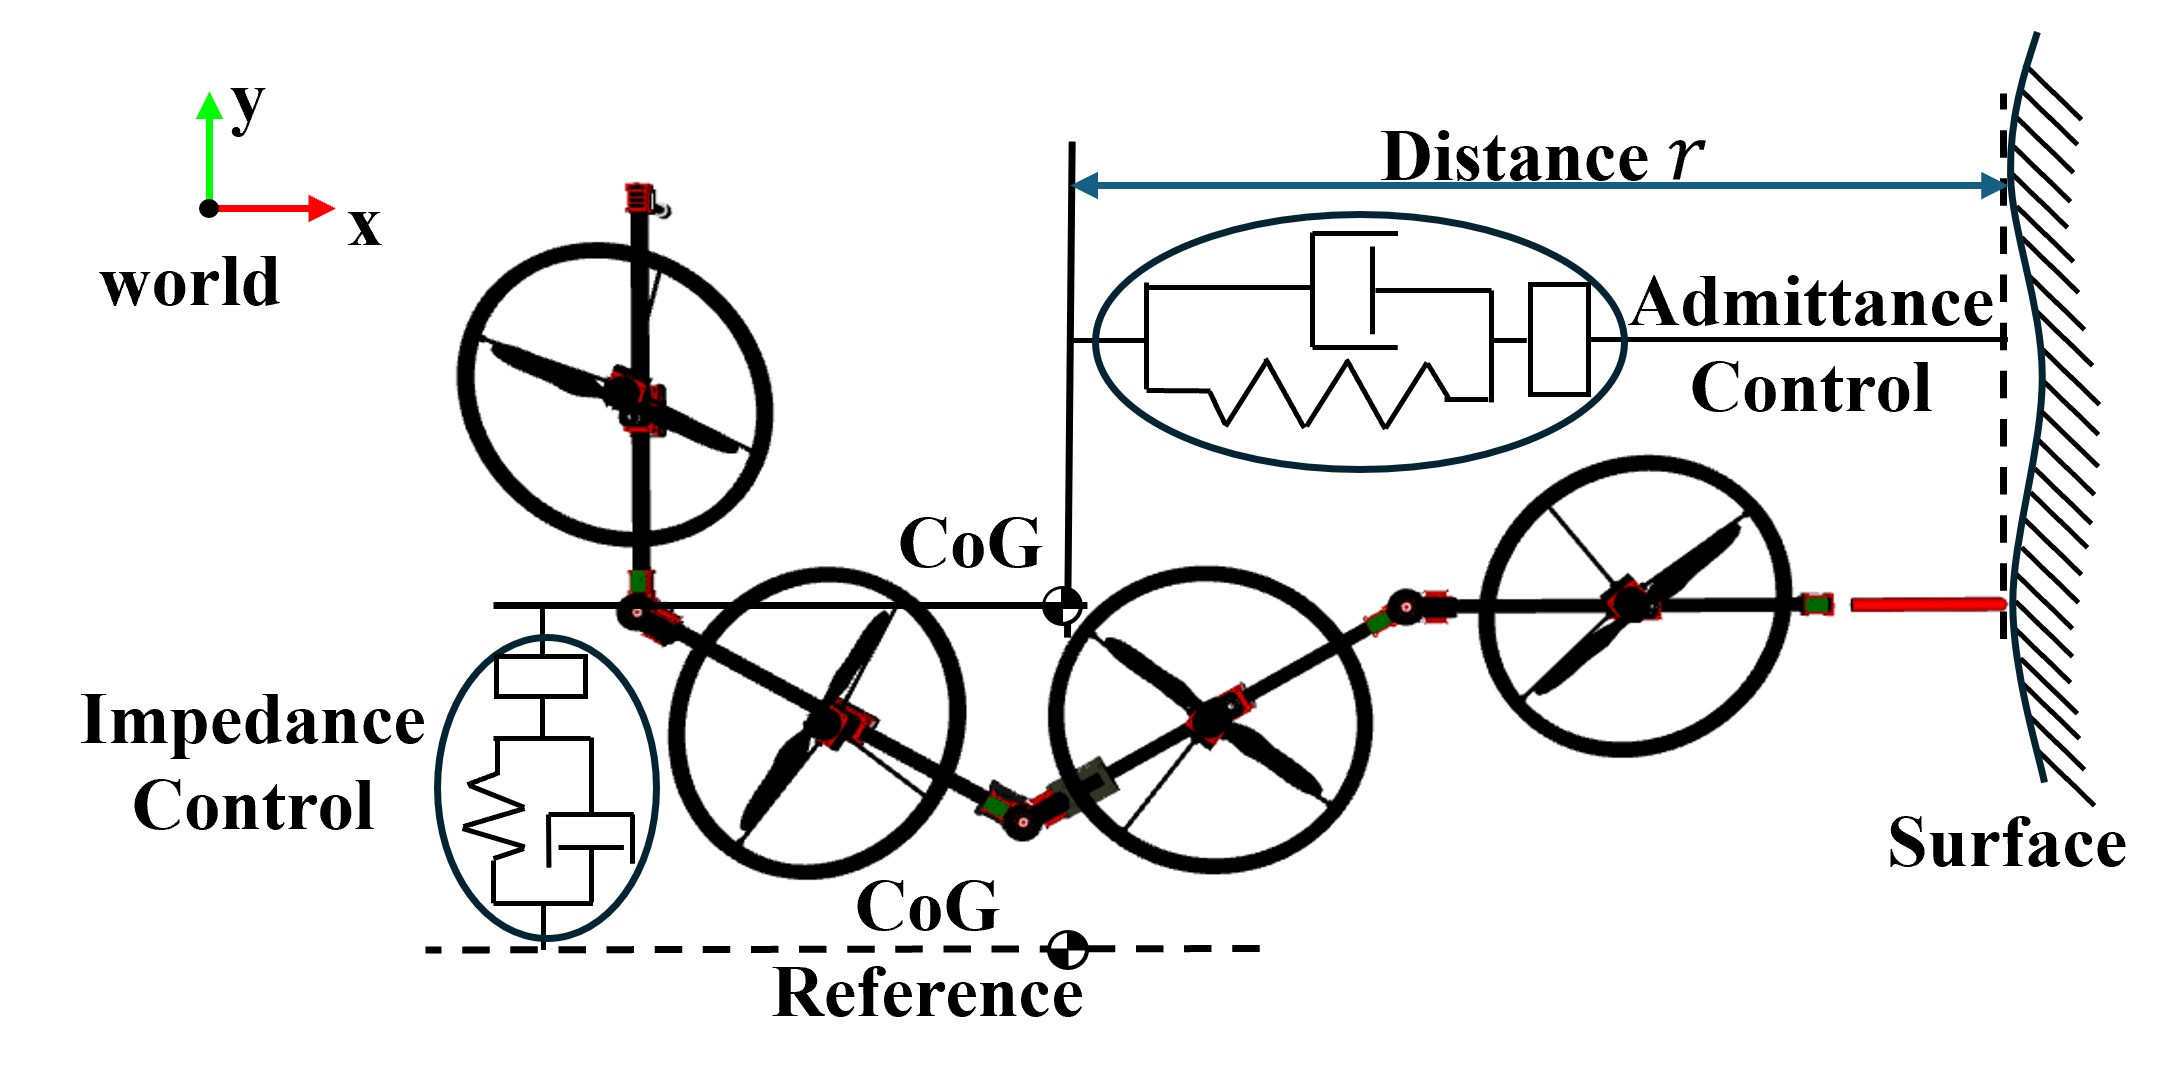
\includegraphics[trim={0cm 0.3cm 0cm 0cm}, clip,width=\linewidth]{figures/chapter3/hybrid.png}
%     \caption{Schematic diagram of the hybrid impedance-admittance control.}
%     \label{fig:hybrid_controller}
%     \vspace{-5mm}
% \end{figure}
\begin{figure}[h]
    \centering
    % \parbox{3in}
    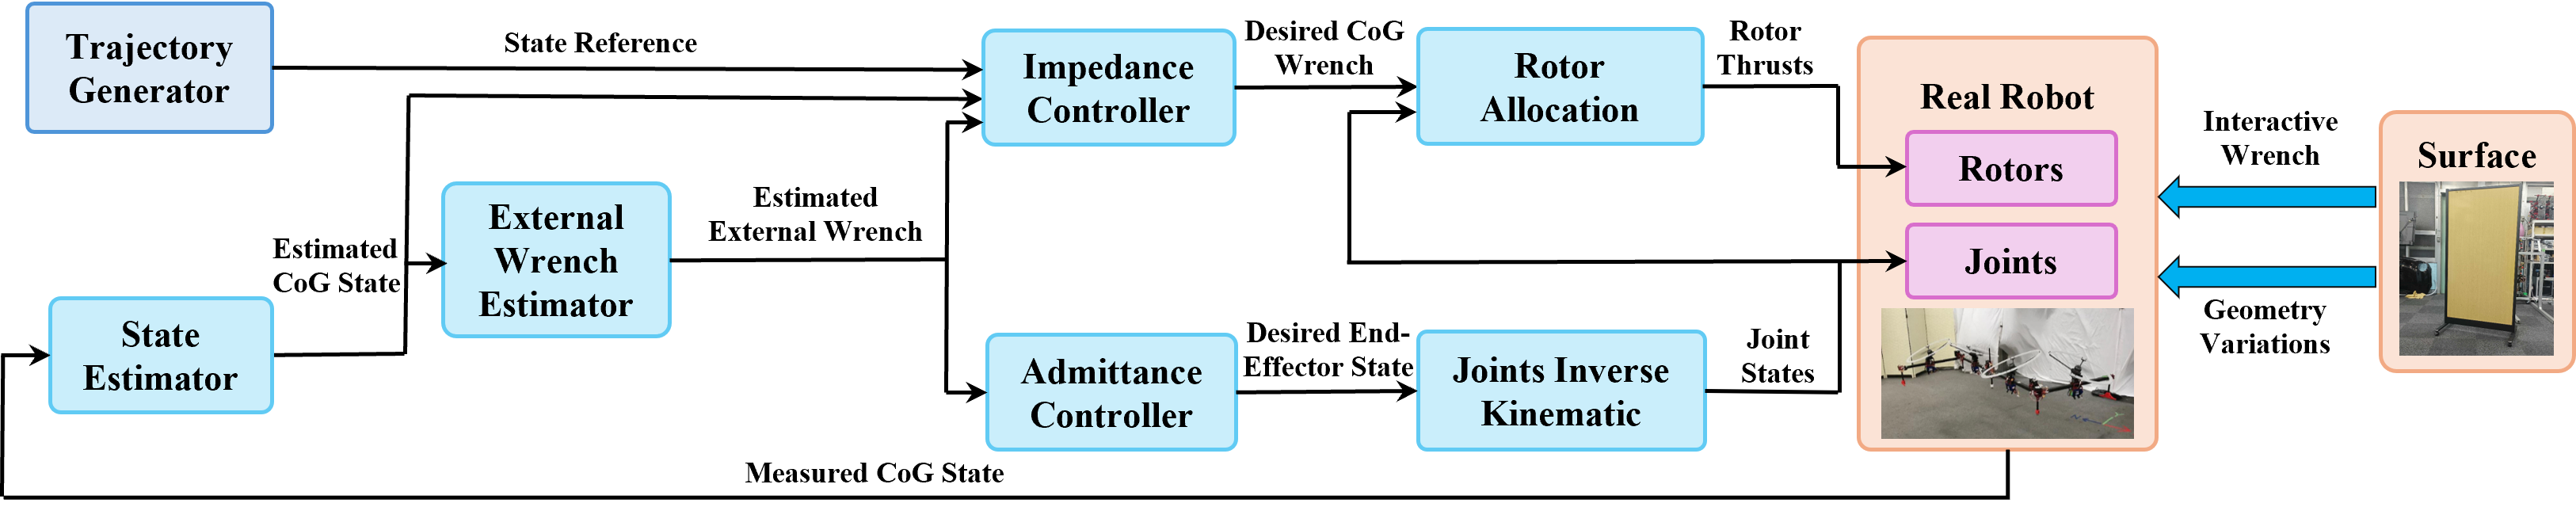
\includegraphics[trim={0cm 0.3cm 0cm 0cm}, clip,width=\linewidth]{figures/chapter3/framework.png}
    \caption{Block diagram of the hybrid impedance-admittance control framework. Inputs for the admittance controller consist of the estimated external wre
    nch. Inputs for the impedance controller include the state reference, estimated CoG state, and estimated external wrench.}
    \label{fig:framework}
    \vspace{-5mm}
\end{figure}

The motivation for this hybrid impedance-admittance control framework is to provide both resilience and adaptivity when sliding on an unknown surface, where geometry and friction introduce significant uncertainties. As illustrated in Fig.~\ref{fig:framework}, impedance control manages the overall state of the aerial robot, which is represented by the pose of its CoG, while admittance control is applied to regulate the end-effector state, resulting in adjustment of the joint angles. Since variations in joint angles modify the robot’s configuration and thus influence the thrust allocation, this dependency is taken into account in the thrust computation.
As illustrated in Fig.~\ref{fig:hybrid_controller}, by combining both controllers, the multi-link aerial robot can regulate its interaction with the surface in both force and position. Detailed analysis of the advantages of this hybrid control is presented in the following section.

%%%%%%%%%%%%%%%%%%%%%%%%%%%%%%%%%%%%%%%%%%%%%%%%%%%%%%%%%%%%%%%%%%%%%%%%%%%%%%%%
\section{External Wrench Estimation}

For both impedance control and admittance control, an external wrench is required in their respective formulations. We can choose to use force sensor to get the measured wrench data, or use estimation method to get a estimated wrench data. Generally, a force sensor is usually could only measure the external wrench applied on where it mounted. On the other hand, the estimation method can deal with force added in anywhere on the aerial robot, but it could distinguish which type of wrench. Considering the framework, the impedance control need to deal with force from different directions added in different point, so we finally choose to use estimated method.

In this framework, a momentum-based external wrench estimation method introduced in \cite{ruggiero_2014_impedance}. The wrench applied at the CoG is obtained as follows:

\begin{subequations}
\label{eq:external wrench estimation}
\begin{align}
 {^W\!\boldsymbol{\tilde{f}}_{ext}}=\boldsymbol{K}_{ti}(m^W\!\dot{\boldsymbol{p}}-\int({^W\!\boldsymbol{f}_{cmd}}-m\boldsymbol{g}+ {^W\!\boldsymbol{\tilde{f}}_{ext}})\mathrm{d}t),\\
 {^C\!\boldsymbol{\tilde{\tau}}_{ext}}=\boldsymbol{K}_{ri}(\boldsymbol{I}^C\!\boldsymbol{\omega}-\int({^C\!\boldsymbol{\tau}_{cmd}}-{^C\!\boldsymbol{\omega}} \times \boldsymbol{I}{^C\!\boldsymbol{\omega}} + {^C\!\boldsymbol{\tilde{\tau}}_{ext}})\mathrm{d}t),
\end{align}
\end{subequations}
where ${^W\!\boldsymbol{\tilde{f}}_{ext}}$ is the estimated external force, ${^C\!\boldsymbol{\tilde{\tau}}_{ext}}$ is the estimated external torque, and they can be assumed to be equal to the real external force ${^W\!\boldsymbol{f}}_{ext}$ and the real external torque   ${^C\!\boldsymbol{\tau}_{ext}}$, respectively. $\boldsymbol{K}_{ti} \in \mathbb{R}^{3\times3} \in $ and $\boldsymbol{K}_{ri} \in \mathbb{R}^{3\times3}$ are the estimator translation gain matrix and estimator rotation gain matrix, respectively.

Differentiating (\ref{eq:external wrench estimation}) and substituting (\ref{eq:dynamics}) into it yields a first-order low-pass filtered form: 
\begin{subequations}
\label{eq:external wrench estimation low-pass}
\begin{align}
 {^W\!\boldsymbol{\dot{\tilde{f}}}_{ext}}&=\boldsymbol{K}_{ti}({^W\!\boldsymbol{f}}_{ext}-{^W\!\boldsymbol{\tilde{f}}_{ext}}),\\
 {^C\!\boldsymbol{\dot{\tilde{\tau}}}_{ext}}&=\boldsymbol{K}_{ri}({^C\!\boldsymbol{\tau}_{ext}}-{^C\!\boldsymbol{\tilde{\tau}}_{ext}}).
\end{align}
\end{subequations}
That means by increasing the parameters, the estimated data will follow the real data faster, but also easier to introduce noise and lead to instability.

Note that \eqref{eq:external wrench estimation} estimates external forces and torques without using acceleration measurements, relying solely on the estimated linear and angular velocities. That means only by using built-in IMU data, we can realize getting the external wrench data.


%%%%%%%%%%%%%%%%%%%%%%%%%%%%%%%%%%%%%%%%%%%%%%%%%%%%%%%%%%%%%%%%%%%%%%%%%%%%%%%%
\section{Impedance Control}
Impedance control models the robot as a second-order system in the sight of environment, so that the robot can adjusting its own movement by external force. To meat different requirements, the dynamic parameters can be freely designed to achieve the desired interaction behavior.
For example, by adjusting the stiffness parameters, the robot can be made resilient in certain directions to reject disturbances while remaining compliant in others to maintain safe interaction \cite{bodie_2020_active}. By using impedance control, we can redesign how the system performs. In this section, we will introduce the normal concept of impedance control, also discuss about the fundamental concept of impedance control, and the difference between the PID control and it. 
% In this section, we will introduce how to adjust parameters to make the aerial robot to meet the require performance.
% In this subsection, we will introduce the 
\subsection{Normal setup}
First we will introduce how to get the command wrench equation of impedance control.
The translational motion is expressed in the world frame $\{W\}$, whereas the rotational motion is expressed in the CoG frame $\{C\}$. Under this convention, the impedance equations are written as:
\begin{subequations}
\label{eq:impedance control 1}
\begin{align}
    {\boldsymbol{M}_{d}}{^W\!\ddot{\boldsymbol{p}}}+{\boldsymbol{C}_{td}}{\boldsymbol{e}_v}+{\boldsymbol{K}_{td}}{\boldsymbol{e}_p}&={^W\!\boldsymbol{\tilde{f}}_{ext}}, \\[2pt]
    {\boldsymbol{I}_{d}}{^C\!\dot{\boldsymbol{\omega}}}+{\boldsymbol{C}_{rd}}{\boldsymbol{e}_\omega}+{\boldsymbol{K}_{rd}}{\boldsymbol{e}_R}&={^C\!\boldsymbol{\tilde{\tau}}_{ext}},
\end{align}
\end{subequations}
where ${\boldsymbol{M}_{d}}\in \mathbb{R}^{3\times3}$ is the desired virtual mass, ${\boldsymbol{I}_{d}}\in \mathbb{R}^{3\times3}$ is the desired virtual inertia, ${\boldsymbol{C}_{td}}\in \mathbb{R}^{3\times3}$, ${\boldsymbol{C}_{rd}}\in \mathbb{R}^{3\times3}$ are the desired linear and rotational damping matrices, and ${\boldsymbol{K}_{td}}\in \mathbb{R}^{3\times3}$, ${\boldsymbol{K}_{rd}}\in \mathbb{R}^{3\times3}$ are the desired linear and rotational stiffness matrices, respectively. All of these matrices are positive definite. These are what we want the system performs like. Here the error vectors in (\ref{eq:impedance control 1}) are defined as:
\begin{subequations}
\label{eq:error of rotation}
\begin{align}
    {\boldsymbol{e}_p}&={^W\!\boldsymbol{p}}-{^W\!\boldsymbol{p}_{ref}}, \\[2pt]
    {\boldsymbol{e}_v}&={^W\!\dot{\boldsymbol{p}}}-{^W\!\dot{\boldsymbol{p}}_{ref}}, \\[2pt]
    {\boldsymbol{e}_R}&=\frac{1}{2}({^W\!\boldsymbol{R}^{\mathrm{T}}_{C,ref}}{^W\!\boldsymbol{R}_{C}}-{^W\!\boldsymbol{R}^{\mathrm{T}}_{C}}{^W\!\boldsymbol{R}_{C,ref}})^\vee, \\[2pt]
    {\boldsymbol{e}_\omega}&={^C\!\boldsymbol{\omega}}-{^W\!\boldsymbol{R}^{\mathrm{T}}_{C}}{^W\!\boldsymbol{\omega}}_{ref},
\end{align}
\end{subequations}
where we use the vee-operator $^\vee$ to extract a vector from a skew symmetric matrix.

Next, by substituting \eqref{eq:dynamics} into \eqref{eq:impedance control 1} to eliminate $\ddot{\boldsymbol{p}}$ and $\dot{\boldsymbol{\omega}}$, the command wrench added on the CoG can be derived. The translational component can be written as

\begin{equation}
\label{eq:imp cmd for trans1}
    {^W\!\boldsymbol{f}_{cmd}}=(m\boldsymbol{M}^{-1}_d-\boldsymbol{E}_3){^W\!\boldsymbol{\tilde{f}}_{ext}}-m\boldsymbol{M}_d^{-1}({\boldsymbol{C}_{td}}{\boldsymbol{e}_v}+{\boldsymbol{K}_{td}}{\boldsymbol{e}_p})+m\boldsymbol{g}.
\end{equation}

And the rotational component can be written as

\begin{equation}
\label{eq:imp cmd for rot1}
    {^{C}\boldsymbol{\tau}_{cmd}}=(\boldsymbol{I}\boldsymbol{I}^{-1}_d-\boldsymbol{E}_3){^{C}}\boldsymbol{\tilde{\tau}}_{ext}-\boldsymbol{I}\boldsymbol{I}^{-1}_d({\boldsymbol{C}_{rd}}{\boldsymbol{e}_\omega}+{\boldsymbol{K}_{rd}}{\boldsymbol{e}_R})+{^{C}\boldsymbol{\omega}} \times \boldsymbol{I}{^{C}\boldsymbol{\omega}}.
\end{equation}
 
\subsection{Parameter tuning discussion}
Apparently, the performance of aerial robot is relied on the parameter matrices. Even though the parameter matrices usually have specific physical meaning, these physical interpretations do not directly provide a practical parameter selection procedure. Therefore, although the qualitative influence of each parameter is generally understood, determining suitable numerical values remains difficult in practice. 

In this thesis, the impedance parameters are analyzed according to the resulting system behavior rather than their physical meanings alone. We can find some relationship between PID control and impedance control, therefore use PID inspired tuning method to find the suitable parameters. We will use 1-dof system to explain it.

Let's consider the following 1-dof impedance control equation
\begin{equation}
\label{eq:imp cmd analysis1}
  m_d\ddot{p}+c_de_v+k_de_p = f_{ext},
\end{equation}
Here, the parameters $m_d$, $c_d$, $k_d$ are the designed mass, the designed damping, and the designed stiffness, respectively. $f_{ext}$ represents the external force.
The dynamic equation of a 1-dof object
\begin{equation}
\label{eq:imp cmd analysis2}
  m\ddot{p}+g(\dot{p}, p) = f_{ext},
\end{equation}
here $g(\dot{p}, p)$ represents an extreme term such as gravity and Coriolis.
By substituting \ref{eq:imp cmd analysis2} into \ref{eq:imp cmd analysis1}, we can get

\begin{equation}
\label{eq:imp cmd analysis3}
{{f}_{cmd}}=(\frac{m}{m_d}-1){{f}_{ext}}-m({\frac{c_d}{m_d}e_v+\frac{c_d}{k_d}e_p})+g(\dot{p}, p).
\end{equation}

Theoretically, the three parameters can be chosen independently refer to the task requirement. 
we define $\tilde{c}_d = \frac{c_d}{m_d}$, $\tilde{k}_d = \frac{k_d}{m_d}$ as the normalized damping and normalized stiffness, respectively. we use $\mu$ to replace $\frac{m}{m_d}$, so the equation becomes 
\begin{equation}
\label{eq:imp cmd analysis4}
{{f}_{cmd}}=(\mu-1){{f}_{ext}}-m({\tilde{c}_de_v+\tilde{k}_de_p})+g(\dot{p}, p).
\end{equation}

If we write the PID control equation 
\begin{equation}
\label{eq:PID cmd}
{{f}_{cmd}}=k_pe_p+k_i\int e_p\mathrm{d}t+k_de_v+g(\dot{p}, p),
\end{equation}
We will find that the two equations are very similar. If we chose $\tilde{c}_d=-\frac{k_d}{m}$ and $\tilde{k}_d=-\frac{k_p}{m}$, the only different lines on the I term $k_i\int e_p\mathrm{d}t$ and the external force term $(\mu-1){{f}_{ext}}$. 

When there exists position error, the I term $k_i\int e_p\mathrm{d}t$ will continue integral to increase the command force. If there is free flight situation, maybe it would not cause problem. But if there exists a non-zero external force, the integral term will increase to infinite except we set a limitation in advance. That is means the integral term unable to respond well to external forces. On the other hand, the external force term $(\mu-1){{f}_{ext}}$ is related to the estimated external force. It can adjust the final command wrench by considering the external force. Therefore, in the contact scenario, it is better to choose impedance control instead of PID control.
% Obviously, they all used for compensate the position errors.
% Let see what will happen in different scenarios. 

However, the impedance control still has a lot of similarities to the PID control. So we can divide it into PD control part and external force part. Apparently, if there is no external force, the external force part should disappear, and only PD control part (also the gravity part which should be considered as feedforward term) left. So we can use PID turning method to find the parameters $\tilde{c}_d$ and $\tilde{k}_d$, now they are consider as the $k_p$ and $k_d$.

After we tuning the parameters in free flight, it must be consider in contact situation. Let us consider the parameter $\mu$. If $\mu$ is set to $0$, the compensation term is exactly the estimated external wrench, so the command will completed compensate the external force. If $\mu$ is set to $1$, the external force term will also disappear, in which situation the impedance controller degenerate to a PD controller. If $\mu >1$, the external force term has the same direction with the external force, so the command will help to push the aerial robot to the direction of external force, which means the aerial robot will follow the external force. In this situation, the aerial robot can be regarded as compliance, the stiffness is relatively low. On the other hand, if $\mu >1$, the external force term has the reverse direction with the external force, which means the command will help to resist the external force. In this situation, the aerial robot will try to reduce its movement at the direction of external force, the stiffness is relatively high. 

In summary, by setting $\mu$ larger or less than $1$, the aerial robot can perform relatively compliant or rigid. By tuning parameters depend on the task requirements and environment situation, the aerial robot can perform differently in each axis. 
% The impedance control usually set the parameter between $0$ and $\inf$. If the parameter

And we can also get the tuning principle as follow. We can first tune $\tilde{c}_d$ and $\tilde{k}_d$ as the PD controller in free flight, the design the value of $\mu$ to realize what the task what to achieve. Because we use the same set of parameters both in free flight and contact, it is not necessary to switch mode before and after contacting.

% This is how we can get the command force and torque.

% The reason we rewrite the equations is that we can consider it in another way.
% The equation can be considered as being consist of three parts: the pure PD control term $-m({\tilde{c}_de_v+\tilde{k}_de_p})$, the compensation term $(\mu-1){{f}_{ext}}$ and the extreme term $g(e_v, e_p)$
So in this insight, the impedance control can be consider as the upper lever of pure PD control and feedforward + PD control, or we can also consider the equation as PID controller whose integral term is replaced by estimated wrench term \cite{bodie_2023_omnidirectional}. If the parameter is set to $1$, the compensation term disappeared, and the equation di to pure PD control. By adjusting $\mu$, the performance will be different, and satisfy the requirements of tasks.





% So actually we use the same parameters whatever the drone is in free flight or in contacting. when contact happen, the equation will use the compensation term to help deal with the external force.
% \eqref{eq:imp cmd for trans1} and 

% If there is static force added in the aerial robot, such as force disturbance. For PID controller, the I term will help to resist the external force, so finally the position errors will disappear. For impedance controller, the external term usually could not completely resist the external force, so there must be position errors remained. But the position error can be reduced by tuning the parameter $\mu$. 
%%%%%%%%%%%%%%%%%%%%%%%%%%%%%%%%%%%%%%%%%%%%%%%%%%%%%%%%%%%%%%%%%%%%%%%%%%%%%%%%
% \section{Parameter analysis}
% In most of the pervious paper using impedance control in aerial manipulation, impedance control is usually used as a tool without being entirely explained. Here we will try to explain it.
% The impedance control equation usually has three parameters to tune. By unit setting, we can rewrite the equation, and discover the insight of the equation.




% %%%%%%%%%%%%%%%%%%%%%%%%%%%%%%%%%%%%%%%%%%%%%%%%%%%%%%%%%%%%%%%%%%%%%%%%%%%%%%%%
% \subsection{Free flight}
% In free flight.
% If there is no force, the two controllers performs similar.
% If there is static force added in the aerial robot, such as force disturbance. For PID controller, the I term will help to resist the external force, so finally the position errors will disappear. For impedance controller, the external term usually could not completely resist the external force, so there must be position errors remained. But the position error can be reduced by tuning the parameter $\mu$. 
% \subsection{Contact}
% In contact state. 
\subsection{Special setup}



Finally, we can rewrite the \ref{eq:imp cmd for trans1} and \ref{eq:imp cmd for rot1} as follow.  Here we define the normalized linear damping and stiffness as $\tilde{\boldsymbol{C}}_{td} = \boldsymbol{M}^{-1}_d\boldsymbol{C}_{td}$ and $\tilde{\boldsymbol{K}}_{td} = \boldsymbol{M}^{-1}_d\boldsymbol{K}_{td}$, respectively. Using these definitions, \eqref{eq:imp cmd for trans1} can be rewritten as
\begin{equation}
\label{eq:imp cmd for trans2}
    {^W\!\boldsymbol{f}_{cmd}}=(m\boldsymbol{M}^{-1}_d-\boldsymbol{E}_3){^W\!\boldsymbol{\tilde{f}}_{ext}}-m(\tilde{\boldsymbol{C}}_{td}{\boldsymbol{e}_v}+{\tilde{\boldsymbol{K}}_{td}}{\boldsymbol{e}_p})+m\boldsymbol{g}.
\end{equation}
Also we define the normalized rotation damping and stiffness as $\tilde{\boldsymbol{C}}_{rd} = \boldsymbol{I}^{-1}_d\boldsymbol{C}_{rd}$ and $\tilde{\boldsymbol{K}}_{rd} = \boldsymbol{I}^{-1}_d\boldsymbol{K}_{rd}$, respectively. Equation (\ref{eq:imp cmd for rot1}) can then be rewritten as
\begin{equation}
\label{eq:imp cmd for rot2}
    {^{C}\boldsymbol{\tau}_{cmd}}=(\boldsymbol{I}\boldsymbol{I}^{-1}_d-\boldsymbol{E}_3){^{C}}\boldsymbol{\tilde{\tau}}_{ext}-\boldsymbol{I}(\tilde{\boldsymbol{C}}_{rd}{\boldsymbol{e}_\omega}+\tilde{\boldsymbol{K}}_{rd}{\boldsymbol{e}_\alpha})
    +{^{C}\boldsymbol{\omega}} \times \boldsymbol{I}{^{C}\boldsymbol{\omega}}.
\end{equation}
Noting that the normalized matrices are considered as contact parameters and are tuned in free flight situation. This is how we get the command wrench.

%%%%%%%%%%%%%%%%%%%%%%%%%%%%%%%%%%%%%%%%%%%%%%%%%%%%%%%%%%%%%%%%%%%%%%%%%%%%%%%%
\section{Admittance Control}
Similar to impedance control, admittance control also regulates the system’s response to external forces through a virtual dynamic relationship. However, impedance control generates a resisting force in response to displacement errors, whereas admittance control directly produces a compliant displacement in response to external forces. In this work, we employ admittance control to regulate the end-effector state by adjusting the joint angles in response to the external forces induced by surface geometric variations, thereby mitigating both the force and position disturbances experienced by the CoG through deformation.  The admittance dynamics can then be written as:


% For the surface-sliding task considered, we define the $x$ axis of the world frame as the contact direction, while the $y$ and $z$ axes represent the sliding directions. Since both the environmental contact forces and geometric variations occur primarily along the contact direction, admittance control is applied only along this direction. The admittance dynamics along the $x$ axis can then be written as:
\begin{equation}
\label{eq:admittance control}
    \boldsymbol{M}_a(\boldsymbol{\ddot{r}}_{ref}-\boldsymbol{\ddot{r}})+\boldsymbol{C}_a(\boldsymbol{\dot{r}}_{ref}-\boldsymbol{\dot{r}})+\boldsymbol{K}_a(\boldsymbol{r}_{ref}-\boldsymbol{r})={\boldsymbol{\tilde{f}}_{ext}}-\boldsymbol{f}_{ref},
\end{equation}
where ${\boldsymbol{\tilde{f}}_{ext}}$ is filtered from ${^W\!\boldsymbol{f}_{ext}}$, and $\boldsymbol{f}_{ref}$ represents the reference external force. The position vector $\boldsymbol{r} \in \mathbb{R}^{3}$ is defined as a distance, the specific definition will be changed due to tasks. The reference position vector $\boldsymbol{r}_{ref}$ corresponds to the original distance.
% , and the reference velocity and acceleration are set as $\dot{r}_{ref}=0$ and $\ddot{r}_{ref}=0$, respectively.
Finally, the parameter diagonal matrices $\boldsymbol{M}_a$, $\boldsymbol{C}_a$, $\boldsymbol{K}_a \in \mathbb{R}^{3\times3}$ denotes the admittance mass, damping, and stiffness in different axes, respectively.

We then employ a discrete-time difference method to compute the distance $\boldsymbol{r}$ at each time step, denoted as $\boldsymbol{r}[k]$. The corresponding acceleration is calculated as: 
\begin{equation}
\label{eq:difference method1}
\boldsymbol{\ddot{r}}[k]=\boldsymbol{M}^{-1}_a(({\boldsymbol{\tilde{f}}_{ext}}-\boldsymbol{f}_{ref})-\boldsymbol{K}_a(\boldsymbol{r}_{ref}-\boldsymbol{r}[k-1])+\boldsymbol{C}_a\boldsymbol{\dot{r}}[k-1]).
\end{equation}
Using this acceleration, the velocity and position can be updated iteratively according to:
\begin{subequations}
\label{eq:difference method2}
\begin{align}
\boldsymbol{\dot{r}}[k]&=\boldsymbol{\dot{r}}[k-1]+\boldsymbol{\ddot{r}}[k]\Delta t, \\[2pt]
\boldsymbol{r}[k]&=\boldsymbol{r}[k-1]+\boldsymbol{\dot{r}}[k]\Delta t,
\end{align}
\end{subequations}
where $\Delta t$ is the control period.

% Given the desired end-effector pose, the corresponding angle $\theta$ that is defined in Fig.~\ref{fig:hybrid_controller} 

Given the desired end-effector pose, the joint angles are obtained by solving the inverse kinematics (IK). This configuration allows external forces to influence the relative distance.
In theory, if we choose appropriate parameters, the distance $r$ will not change rapidly, which will help to keep stable.

Actually, consider we just what to realize displacement follow by force, we can choose to change linearly. But due to the effect of admittance control, it is adjustable by changing the parameters, which means that in different situation, we can provide different performance by tuning the parameters.




%%%%%%%%%%%%%%%%%%%%%%%%%%%%%%%%%%%%%%%%%%%%%%%%%%%%%%%%%%%%%%%%%%%%%%%%%%%%%%%%
\section{Validation on Hydrus}
\subsection{Impedance control on Hydrus}
To use impedance control on Hydrus, we need do some special step. Due to Hydrus is an underactuated system, it must control the translation part and rotation part cascadely.
To obtain the desired thrust vector, we first calculate the translational command force magnitude by
\begin{equation}
\label{eq:thrust translation 1}
    f_{cmd}=(^W\!\boldsymbol{R}_{C}\boldsymbol{b}_3){^W\!\boldsymbol{f}_{cmd}},
\end{equation}
where $^{W}\boldsymbol{R}_{C}\boldsymbol{b}_3$ represents the unit vector along the $z$ axis of the CoG frame expressed in the world frame.

Next, we determine the thrust vector associated with the rotational component. By using the tranlational command, the desired roll angle $^W\!\alpha^{tgt}_x$ and desired pitch angle $^W\!\alpha^{tgt}_y$ are computed as
\begin{subequations}
\label{eq:target roll and pitch angle}
\begin{align}
    {^W\!\alpha^{tgt}_x}&=atan^{-1}(-{^W\!\bar{f}_{y,cmd}},\sqrt{{^W\!\bar{f}_{x,cmd}^2}+{^W\!\bar{f}_{z,cmd}^2}}), \\[2pt]
    {^W\!\alpha^{tgt}_y}&=atan^{-1}(^W\!\bar{f}_{x,cmd},{^W\!\bar{f}_{z,cmd}}),
\end{align}
\end{subequations}
where
\begin{equation}
\label{eq:imp cmd for trans}
    \begin{bmatrix}
^W\!\bar{f}_{x,cmd} & ^W\!\bar{f}_{y,cmd} & ^W\!\bar{f}_{z,cmd}
\end{bmatrix}^{\mathrm{T}}=R^{-1}_Z(^W\!\alpha_z)^W\!\boldsymbol{f}_{cmd}.
\end{equation}
Here, $R_Z(\cdot{})$ is a rotation matrix that only rotates along the $z$ axis with a certain angle.

Employing the computed target roll $^W\!\alpha^{tgt}_x$, target pitch $^W\!\alpha^{tgt}_y$, and the reference yaw angle $^W\!\alpha^{ref}_z$, the reference rotation matrix $^W\!R_{C,ref}$ in \eqref{eq:error of rotation} is constructed, from which the rotation error vector ${\boldsymbol{e}_R}$ is derived. 
% In near hovering condition, we also define ${\boldsymbol{e}_\alpha}$ as the vector form of ${\boldsymbol{e}_R}^\wedge$, where the hat operator $^\wedge$ converts a skew-symmetric matrix into its corresponding vector representation.

Next, we define the following allocation relationship:
\begin{equation}
\label{eq:thrust translation 2}
     \begin{bmatrix} mf_{cmd}&0&0&0\end{bmatrix}^{\mathrm{T}}=\begin{pmatrix}
\boldsymbol{Q}_{tz} \\
\boldsymbol{Q}_r
\end{pmatrix}\boldsymbol{\lambda}_t,
\end{equation}
where $\boldsymbol{Q}_{tz} \in \mathbb{R}^{1 \times 4}$ is the third row of $\boldsymbol{Q}_t$. Solving \eqref{eq:thrust translation 2} yields the translational thrust vector $\boldsymbol{\lambda}_t$. Note that the purpose of the translational command force is to counteract gravity and generate the required translational acceleration, while ensuring that it does not affect the rotational direction.

Then the rotation thrust vector can be obtained by
\begin{equation}
\label{eq:thrust rotation 1}
     \boldsymbol{\lambda}_r=\boldsymbol{Q}_r^{\dagger}{^{C}\boldsymbol{\tau}_{cmd}},
\end{equation}
where $\boldsymbol{Q}_r^{\dagger}$ is the Moore–Penrose pseudoinverse of $ \boldsymbol{Q}_r$.

Finally, the total thrust required to be generated by the rotors can be obtained as
\begin{equation}
\label{eq:thrust}
\boldsymbol{\lambda}=\boldsymbol{\lambda}_t+\boldsymbol{\lambda}_r,
\end{equation}
This gives the individual thrust values that each rotor needs to produce. 
% The detail calculated of allocation process about the thrusts can be found in \cite{zhao_2021_singularity}.

\subsection{Admittance control on Hydrus}
In Hydrus's case, we only test one direction. For the surface-sliding task considered in this study, the $x$ axis of the world frame is defined as the contact direction, while the $y$ and $z$ axes represent the sliding directions. Since the geometric variations occur primarily along the contact direction, only single-axis admittance control is employed along this direction. This design choice avoids additional structural motions in non-contact directions, which could adversely affect the stability of the aerial robot. The admittance dynamics along the $x$ axis can then be written as: 
\begin{equation}
\label{eq:admittance control2}
    m_a(\ddot{r}_{ref}-\ddot{r})+c_a(\dot{r}_{ref}-\dot{r})+k_a(r_{ref}-r)=\hat{f}_{ext,x}-f_{ref,x},
\end{equation}

\begin{equation}
\label{eq:difference method1}
\ddot{r}[k]=\frac{(\hat{f}_{ext,x}-f_{ref,x})-k_a(r_{ref}-r[k-1])+c_a\dot{r}[k-1]}{m_a}.
\end{equation}
Using this acceleration, the velocity and position can be updated iteratively according to:
\begin{subequations}
\label{eq:difference method2}
\begin{align}
\dot{r}[k]&=\dot{r}[k-1]+\ddot{r}[k]\Delta t, \\[2pt]
r[k]&=r[k-1]+\dot{r}[k]\Delta t,
\end{align}
\end{subequations}

Consequently, variations in surface geometry induce corresponding changes in the contact forces. Due to the adoption mechanism,  the majority of geometric variations and external force disturbances are absorbed at the joints, while the portion transmitted to the CoG is significantly reduced, leading to more favorable overall motion behavior of the aerial robot.
As shown in Fig.~\ref{fig:admittance_config}, we set the 2D multi-link aerial robot as the configuration to test the admittance effect. There is a rope attach at leg in joint$2$. By pulling the rope, we can imitate a external force on the negative direction of $x$ axis. As shown in Fig.~\ref{fig:admittance_changing}, the multi-link structure will change due to the external force. Fig.~\ref{fig:hybrid_controller} shows the relationship between the external force and the distance between the end effector and the CoG.


\begin{figure}[h]
    \centering
    % \parbox{3in}
    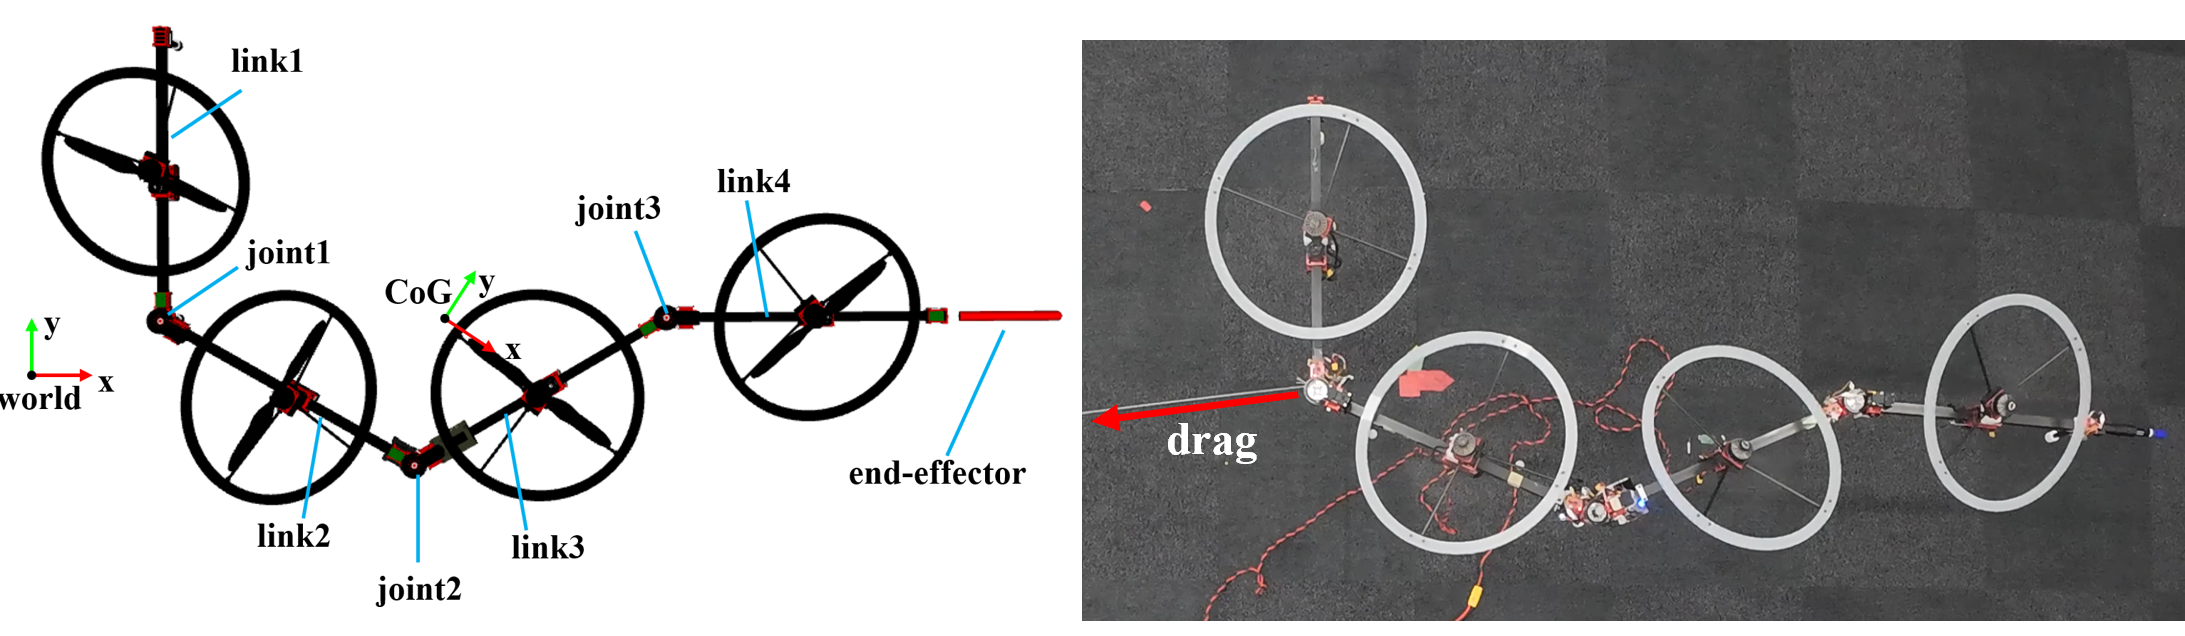
\includegraphics[trim={0cm 0.3cm 0cm 0cm},clip,width=\linewidth]{figures/chapter3/admittance_config.png}
    \caption{Admittance example configuration. Left, the model example. Right, the real machine.}
    \label{fig:admittance_config}
    \vspace{-5mm}
\end{figure}

\begin{figure}[h]
    \centering
    % \parbox{3in}
    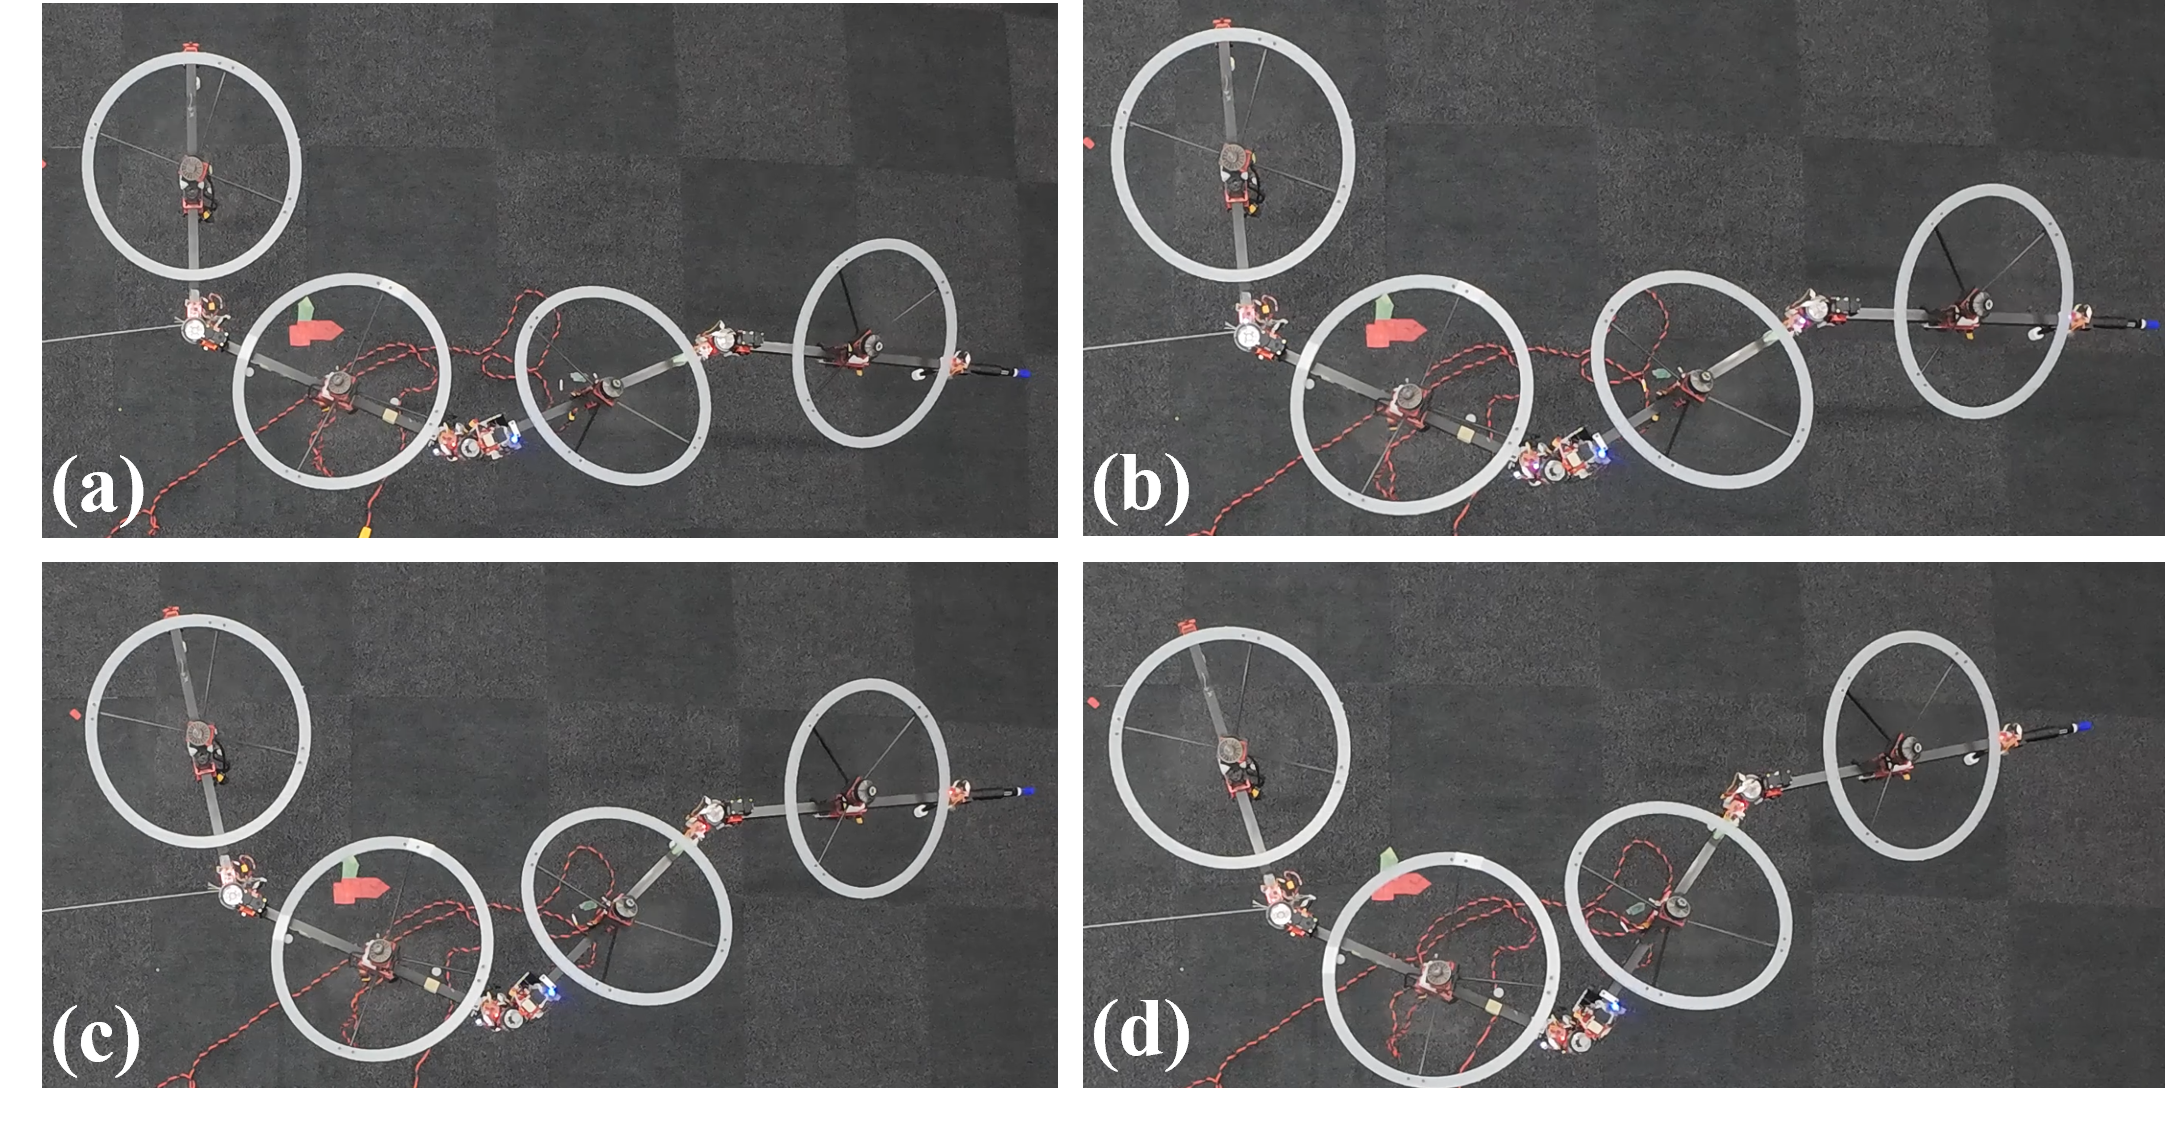
\includegraphics[trim={0cm 0.3cm 0cm 0cm},clip,width=\linewidth]{figures/chapter3/admittance_changing.png}
    \caption{(a)-(d): Admittance changing process.}
    \label{fig:admittance_changing}
    \vspace{-5mm}
\end{figure}

\subsection{Hybrid Control Mechanism} 

In surface-sliding tasks, the contact and sliding directions exhibit fundamentally different physical characteristics: the sliding directions are dominated by friction-induced disturbances, whereas the contact direction is shaped by geometric variations of the environment. Leveraging this distinction, the hybrid impedance–admittance controller assigns each axis the control behavior best suited to its interaction properties. As illustrated in Fig.~\ref{fig:hybrid_controller}, admittance control is applied along the contact direction ($x$ axis) to regulate geometry-driven variations, while impedance control governs the sliding directions ($y$ and $z$ axes) to accommodate friction-affected motion.

Through this task-aligned division of control responsibilities, the hybrid controller achieves what neither controller can provide alone: robust sliding performance in the sliding directions and adaptive behavior in the contact direction. This directional decomposition is enabled by the actuation structure of the multi-link aerial robot, which allows the two control paradigms to be realized simultaneously through independent actuation sources. This combination is therefore essential for achieving resilient interaction and adaptive contact behavior in surface-sliding tasks. The performance of the proposed hybrid impedance-admittance controller will be exhibited in the experiment chapter.

\begin{figure}[h]
    \centering
    % \parbox{3in}
    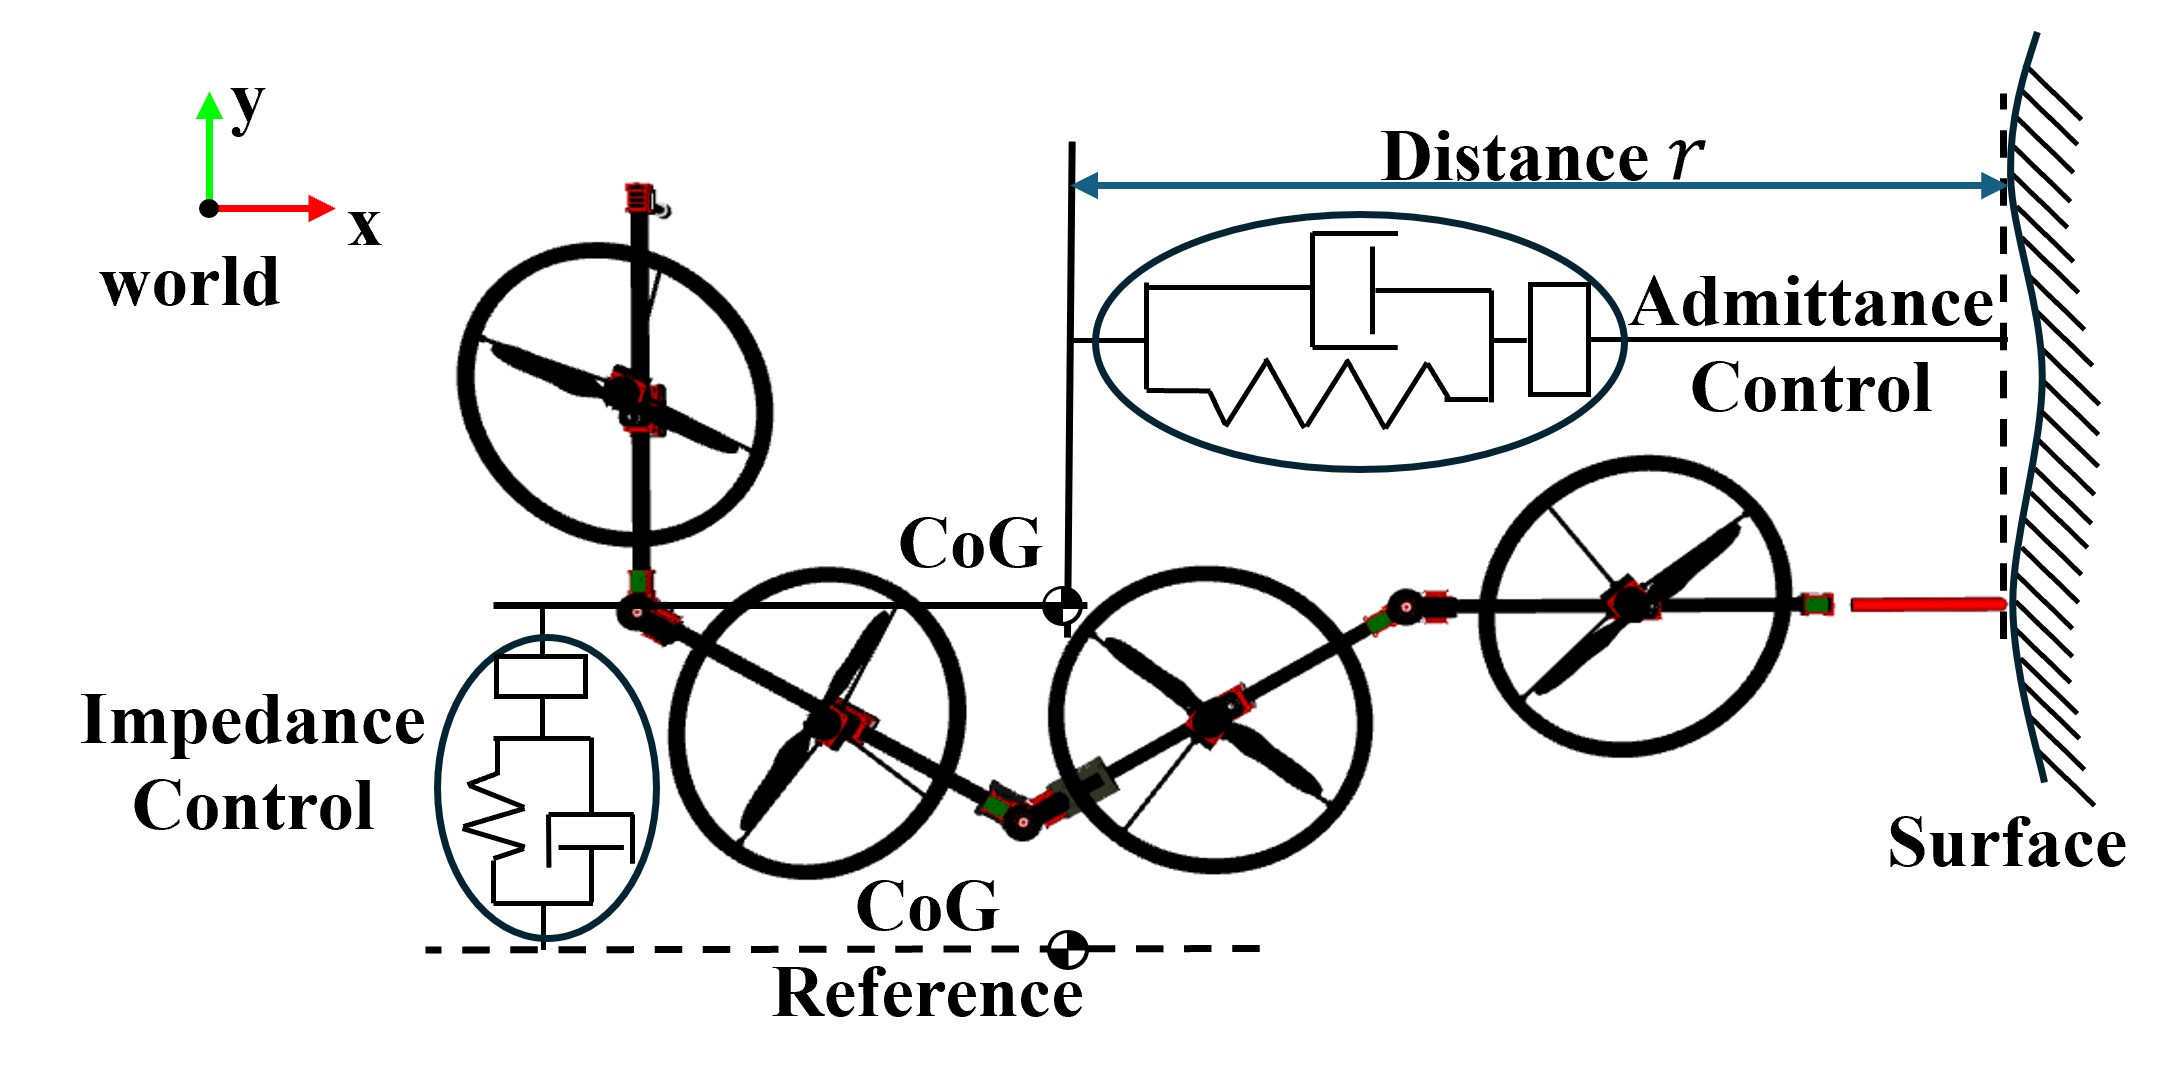
\includegraphics[trim={0cm 0.3cm 0cm 0cm},clip,width=\linewidth]{figures/chapter3/hybrid.png}
    \caption{Schematic diagram of the hybrid impedance-admittance control.}
    \label{fig:hybrid}
    \vspace{-5mm}
\end{figure}

%%%%%%%%%%%%%%%%%%%%%%%%%%%%%%%%%%%%%%%%%%%%%%%%%%%%%%%%%%%%%%%%%%%%%%%%%%%%%%%%
\section{Summary}
In this chapter. We explain that the impedance control can help to change the dynamics parameters of the system, in order to have different performances in different directions. Also, the admittance control can help to adjust the distance between the end-effector and a reference point(es tl. CoG) on the aerial robot, and help to adapt to the geometric variation of the surface. Finally, we explain both the controllers can be added together on the multi-link aerial robot and achieve the surface sliding tasks.
\include{4_integration}
\include{5_experiment}
\include{6_conclusion}
\chapter*{Acknowledgements}
\addcontentsline{toc}{chapter}{Acknowledgements}

The two years since I entered the University of Tokyo have passed very quickly. Although I experienced a lot of difficulties and stress during this period, I also learned and gained a lot, both academically and personally. All these experiences have become an important part of my life. I would like to express my gratitude to all the people who supported me during this period.

First, I would like to express my sincere gratitude to my supervisor, Lecturer Moju Zhao (Chou sensei), for his careful guidance. His guidance opened the door for me to reach a higher academic level and greatly improved my academic and engineering abilities. I especially enjoyed our research discussions. You always patiently listened to my long explanations and provided valuable insights. These discussions also gave me great encouragement. Beyond research, I am also grateful for your concern about my personal situation and for the opportunity to work as a research assistant. It has been my great honor to study under your supervision.

Next, I would like to express my gratitude to all the members of DRAGON Lab. I received a lot of academic support and advice from the senior members, especially for my research and the conference paper. I also had opportunities to help some junior members with their research, from which I learned a lot as well. Beyond research, I enjoyed the time we spent together at parties and playing games. Communicating with members from different countries also gave me opportunities to experience different cultures and improve my communication skills. Their support brought me some relief during stressful periods, and the time we spent together became an important part of my life at the University of Tokyo.

I would also like to thank several friends of mine who have given me a lot of support, and the team where we met and shared many valuable experiences during my undergraduate years. The experience there helped me build my academic and engineering foundations and was also the main reason why I became interested in robotics. After a long and tough period, I am very glad to see the great development of the team during these two years. Their efforts and achievements have also given me encouragement in my own study and research. I sincerely wish the team all the best for its future development.

Finally, I would like to express my sincere gratitude to my parents for their continuous financial and emotional support. Their support gave me the opportunity and confidence to study abroad, and their encouragement helped me during some difficult periods. During these two years, I also learned to pay more attention to how I communicate and get along with my family. This change made me realize and value my own personal growth. I am deeply grateful for your understanding and support throughout my studies.


\begin{flushright}
Zicheng Luo

Aug. 17th, 2026
\end{flushright}
\bibliographystyle{bib/IEEEtransBST/IEEEtran}
\bibliography{bib/reference}



% 後書き
\backmatter
\appendix

\printindex
\end{document}